\section{Evaluation}~\label{sec:evaluation}

In this section, we empirically evaluate our techniques against other \pr clause
learning techniques. In doing so, we aim to answer the following research questions:


\begin{enumerate}
    \item Can our approach provide short \pr proofs for certain benchmark families?
    \item Is our approach less sensitive to encoding choices compared to other
    \pr learning techniques?
    % \item Can these techniques underperform or outperform SAT solvers on other certain benchmark
    % families?
\end{enumerate}


We compare the two main tools learning \pr: clauses \sadical (based on SDCL)
and \prelearn (a preprocessing technique that calls \sadical). To be consistent with our approach,
we run \prelearn with 50 iterations and for 30 seconds. We also compare to \cadical as a baseline with no \pr clause learning.

All experiments were performed in the Anvil Supercomputing Center on nodes with
128 cores and 2 GB RAM per core~\cite{anvil}. We ran 64 experiments in parallel per node
with a 5,000 second timeout, the default timeout for the SAT competition.

In \autoref{subsec:eval-pigeonhole}, we compare all approaches
on the pigeonhole principle, evaluating runtime, proof length, and sensitivity to the encoding of the formula. 
In \autoref{subsec:eval-satcomp}, we evaluate the solvers on benchmarks from the
annual '22, '23, and '24 SAT competition's main 
tracks~\cite{satcomp2022,satcomp2023,satcomp2024}. 
In \autoref{subsec:eval-discussion}, we highlight certain benchmark families
that benefit from \pr clause learning. %We evaluate the different approaches on these families. 
Finally, we analyze the use of specific heuristic choices in \tool
by turning heuristics off individually and observing their effect (\autoref{subsec:eval-heuristics}). 



\subsection{Pigeonhole results}~\label{subsec:eval-pigeonhole}

\begin{figure*}[!t]
    \centering
    \begin{subfigure}[t]{0.4\textwidth}
        \centering
        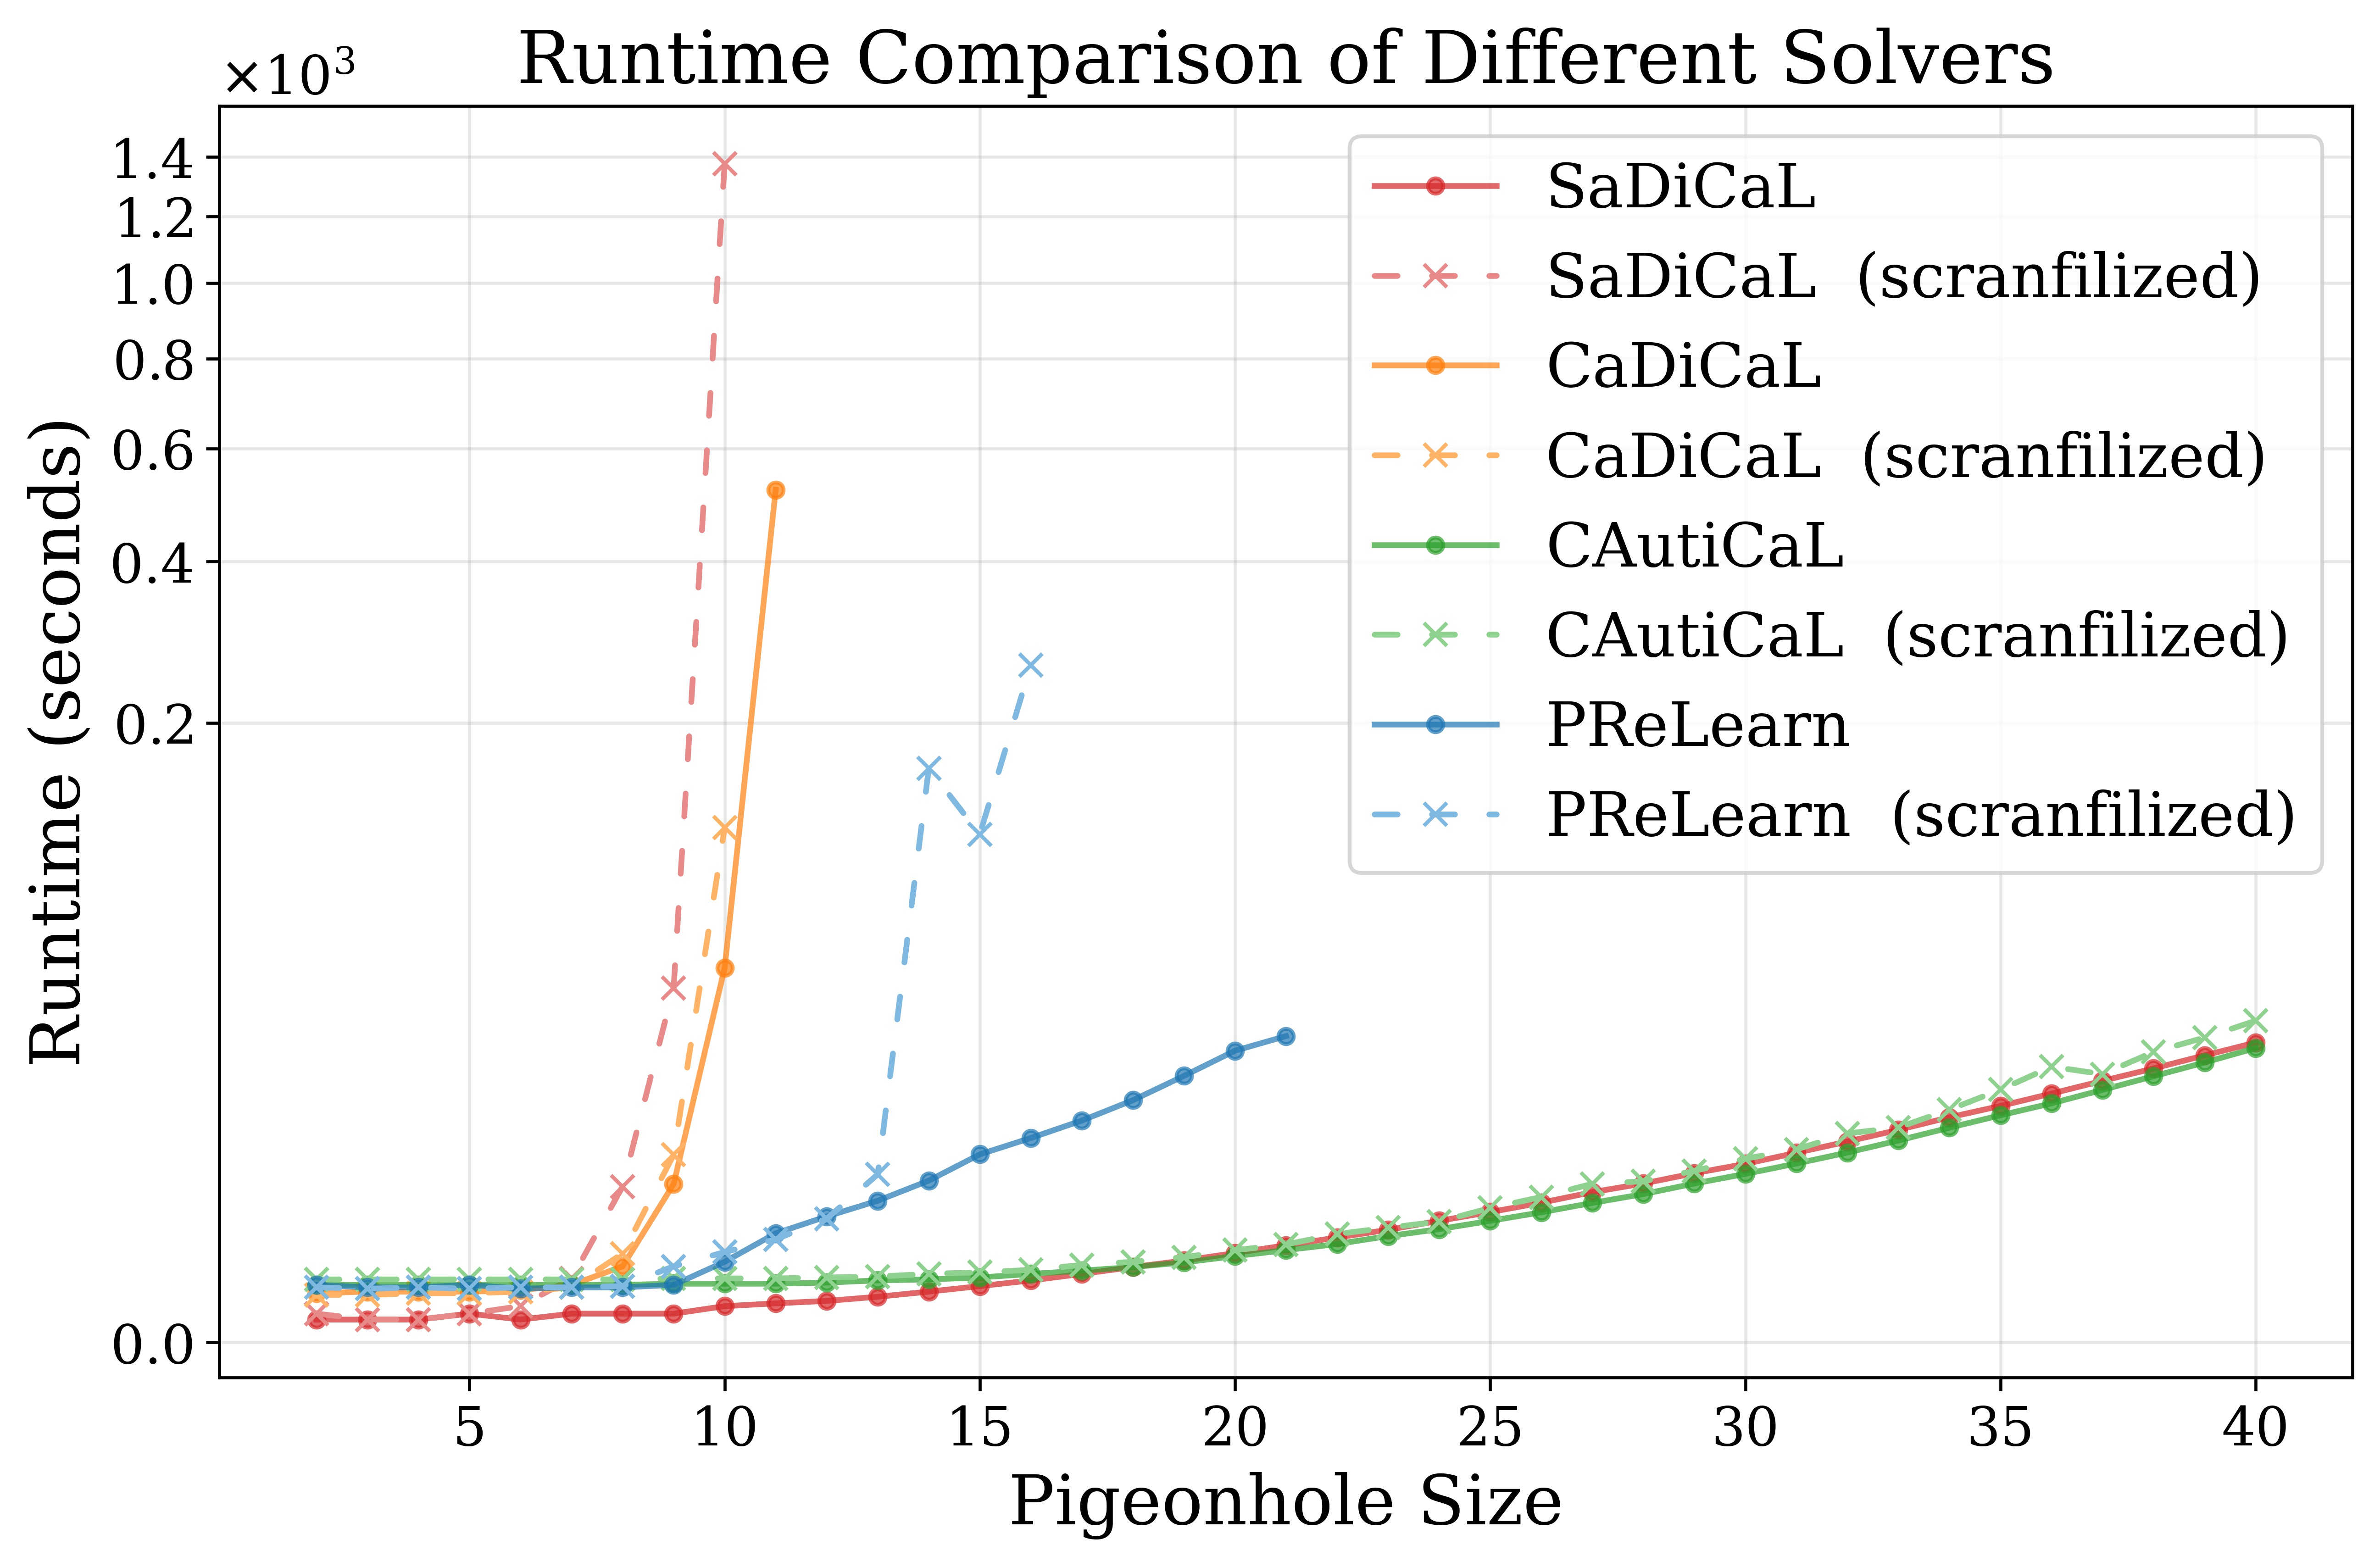
\includegraphics[width=\textwidth]{figs/pigeonhole_runtime_comparison.jpg}
        % \caption{Runtime on Pigeonhole Principle formulae}
        \label{fig:pigeonhole-runtime-comparison}
    \end{subfigure}
    \hspace{0.06\textwidth}
    \begin{subfigure}[t]{0.4\textwidth}
        \centering
        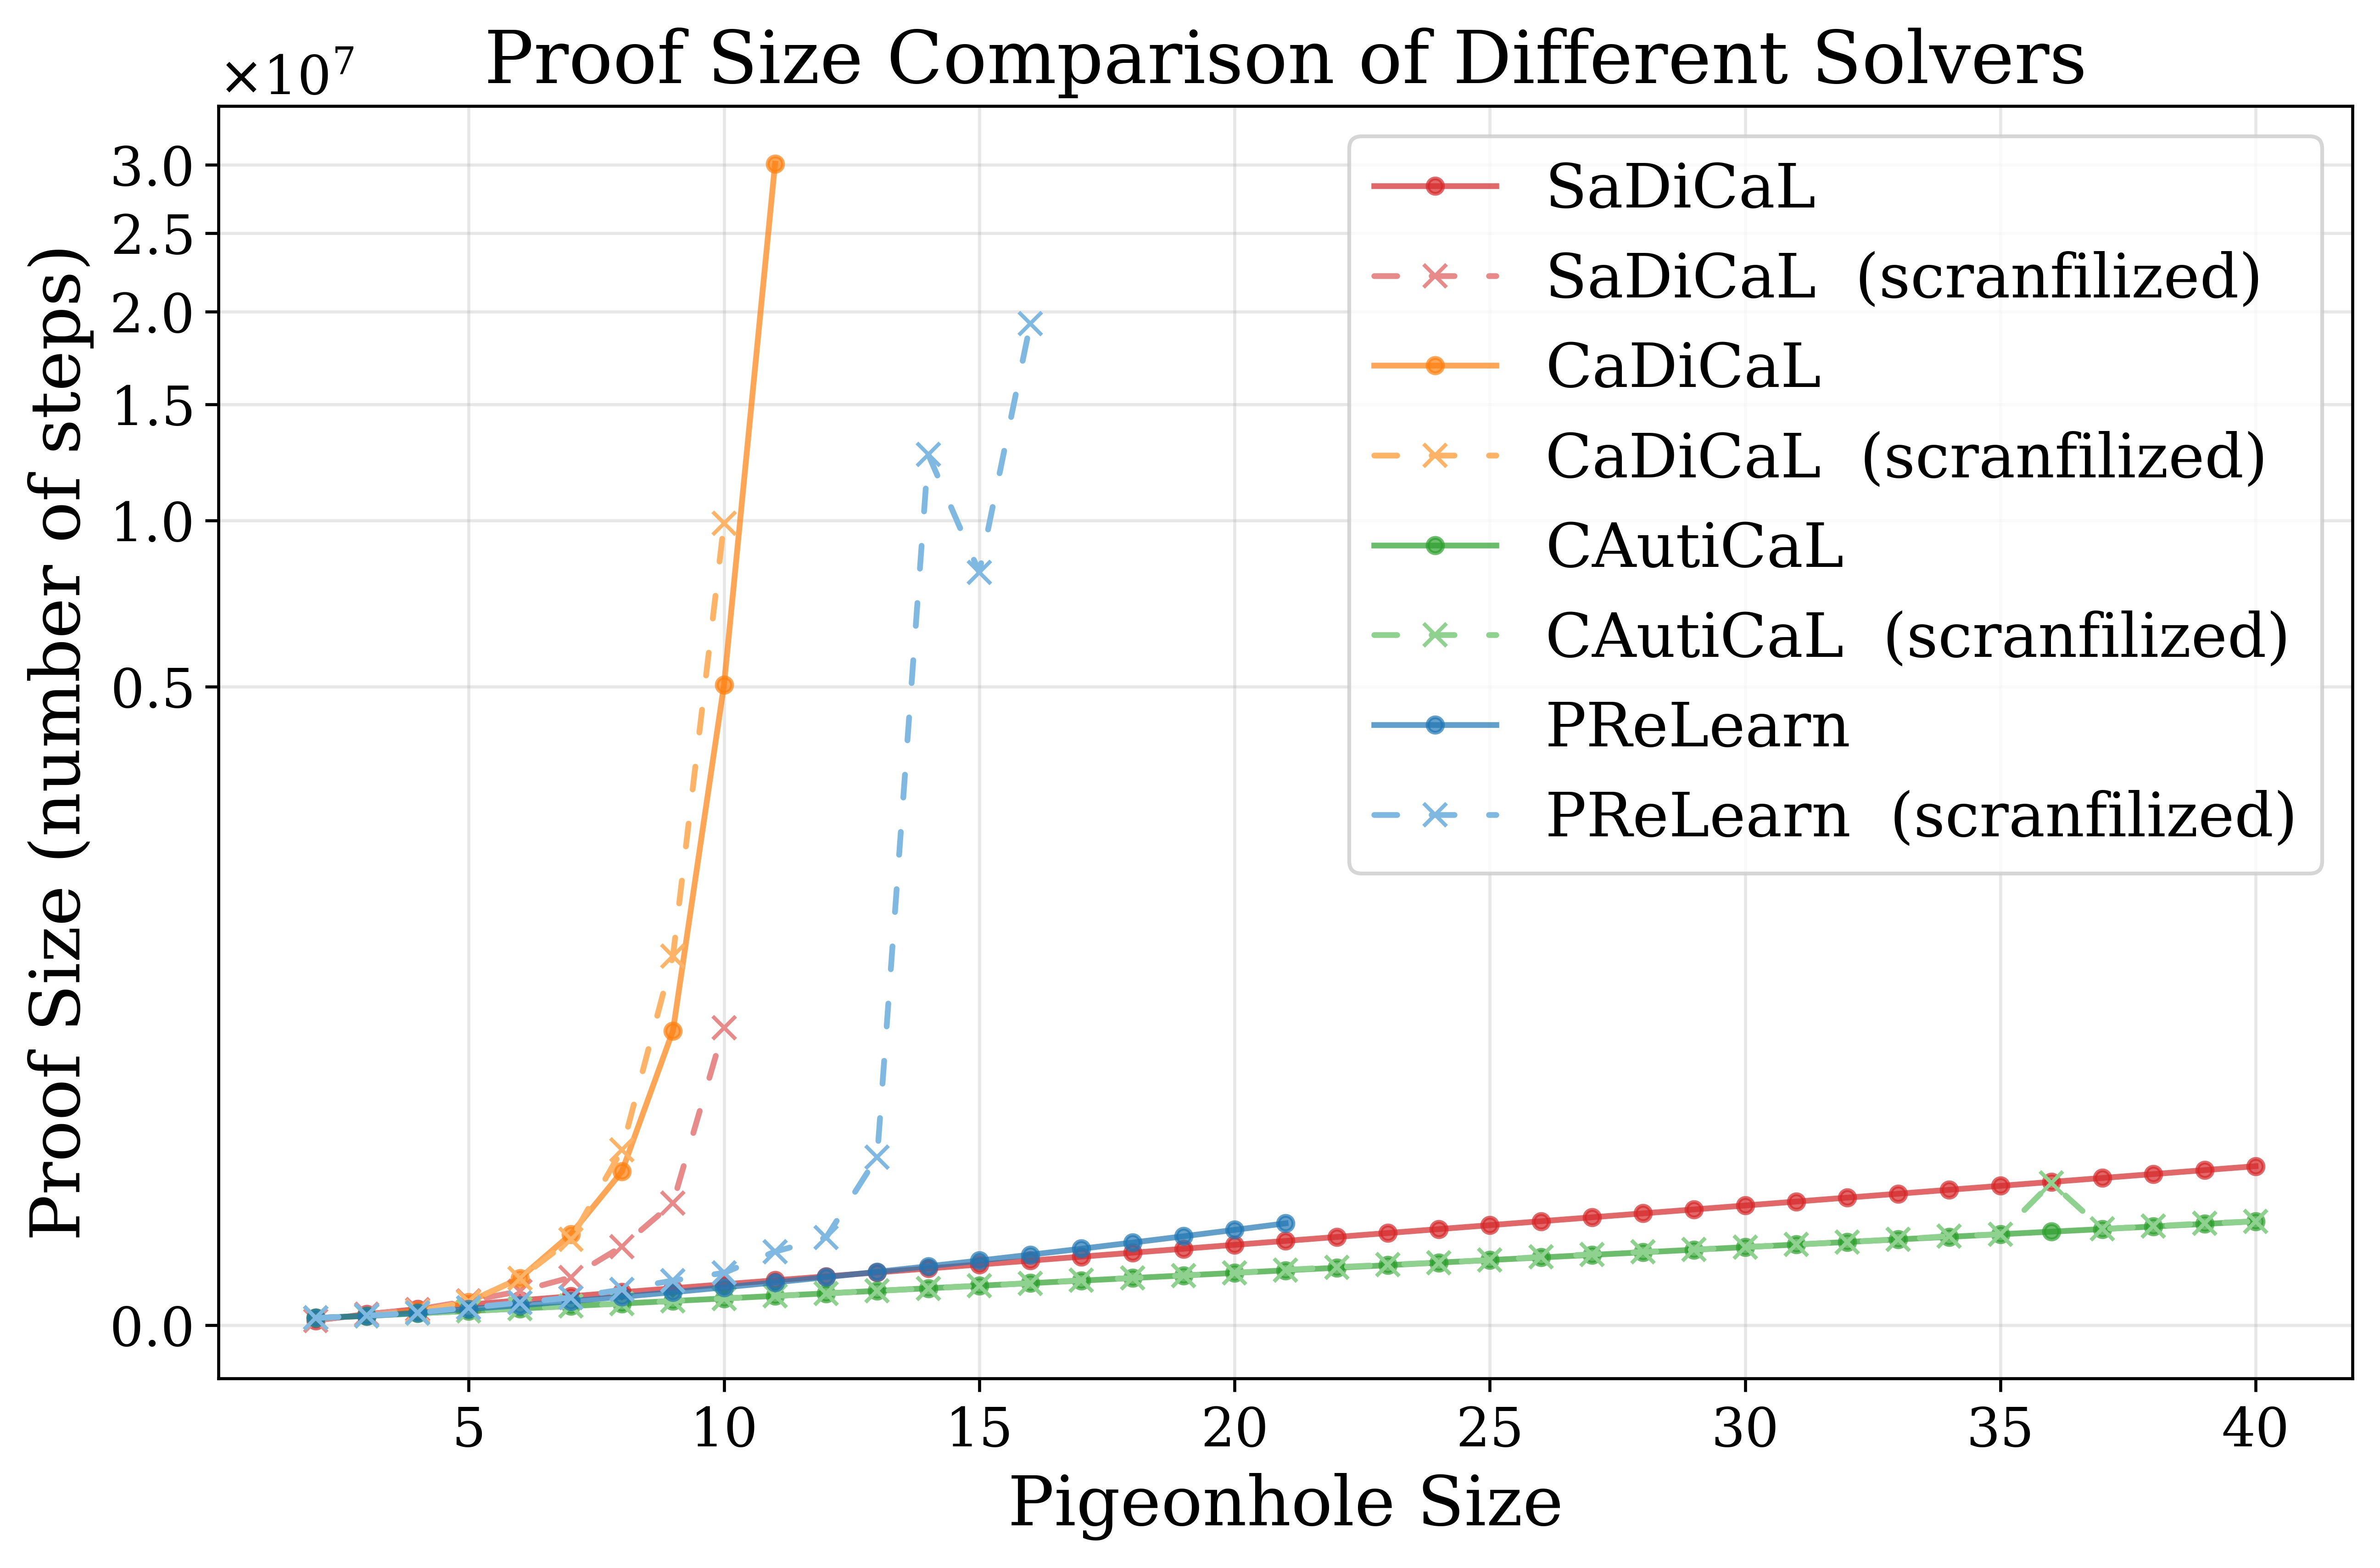
\includegraphics[width=\textwidth]{figs/pigeonhole_proof_size_comparison.jpg}
        % \caption{Proof Size for Pigeonhole Principle formulae}
        \label{fig:pigeonhole-proof-size-comparison}
    \end{subfigure}
    \caption{Comparison of \tool, \cadical, \sadical, and \prelearn on pigeonhole principle benchmarks up to size $40$. The y-axis is on a cube root scale. The performance of a solver on the original benchmark is shown with a solid line. The median of 5 scranfilized queries is shown with a dashed line. If a solver times out on a query in 5000s, it is not shown.}
    \label{fig:pigeonhole-results}
\end{figure*}


Approaches based on SDCL, such as \sadical, are successful for learning $O(n^3)$ proofs for the pigeonhole
principle, but are very sensitive to the encoding of the formula. We compare the solvers on
pigeonhole principle from \ph{2} to \ph{40} and plot these results in \autoref{fig:pigeonhole-results}. As the expected best-behavior is cubic, we use a cube root scale for the y-axis.

As expected, \cadical grows exponentially, while \sadical and \tool scale cubicly in both runtime and proof size. Significantly, \tool is able to learn $3.59$-$3.64$x shorter proofs compared to \sadical. 
% on formulae larger than \ph{10}
This is because \sadical deletes clauses more frequently, as to not exclude other clauses from being learned. Frequent deletion is not necessary in \tool because of its clause shrinking technique.
\prelearn scales cubicly on small formulae, but for \ph{22} and larger, will not learn enough useful \pr clauses in the preprocessing step and times out.

% As we discuss in
% \autoref{app:pigeonhole}, \tool learns proofs of size $\approx \frac13 n^3$,
% which is expected to be shorter than known \pr proofs for the pigeonhole principle.

Additionally, we evaluate all solvers on scranfilized variations of the
pigeonhole principle. Scranfilization is a technique for generating an
equivalently satisfiable formula~\cite{scranfilize}. We use the tool
\texttt{scranfilize}~\cite{scranfilize} with the options permuting variables, permuting clauses, and flipping literals (with probability $0.5$) all turned on. We run each solver on 5 scranfilized variations for
each benchmark and take the median runtime and proof size. This is shown in \autoref{fig:pigeonhole-results} with dashed lines.

\sadical and \prelearn exhibit an exponential trend for runtime and proof size on the scranfilized benchmarks. \sadical will spend all its time in the main SDCL loop not learning enough useful clauses. \prelearn will learn some useful \pr clauses in preprocessing, but not enough to sufficiently shrink the search space for formulae larger than \ph{16}.

On the other hand, \tool almost matches its non-scranfilized performance, demonstrating that it learns useful \pr clauses regardless of the encoding.

% In conclusion, \tool is able to match \sadical's runtime for the pigeonhole principle while shorter proofs by a constant factor. Additionally, \tool is insensitive to permuting variables, permuting clauses, and flipping literals as it relies on conditional autarkies, a global property of the formula.



\subsection{SAT competition results}~\label{subsec:eval-satcomp}

\begin{figure*}[!t]
    \centering
    \begin{subfigure}[t]{0.45\textwidth}
        \centering
        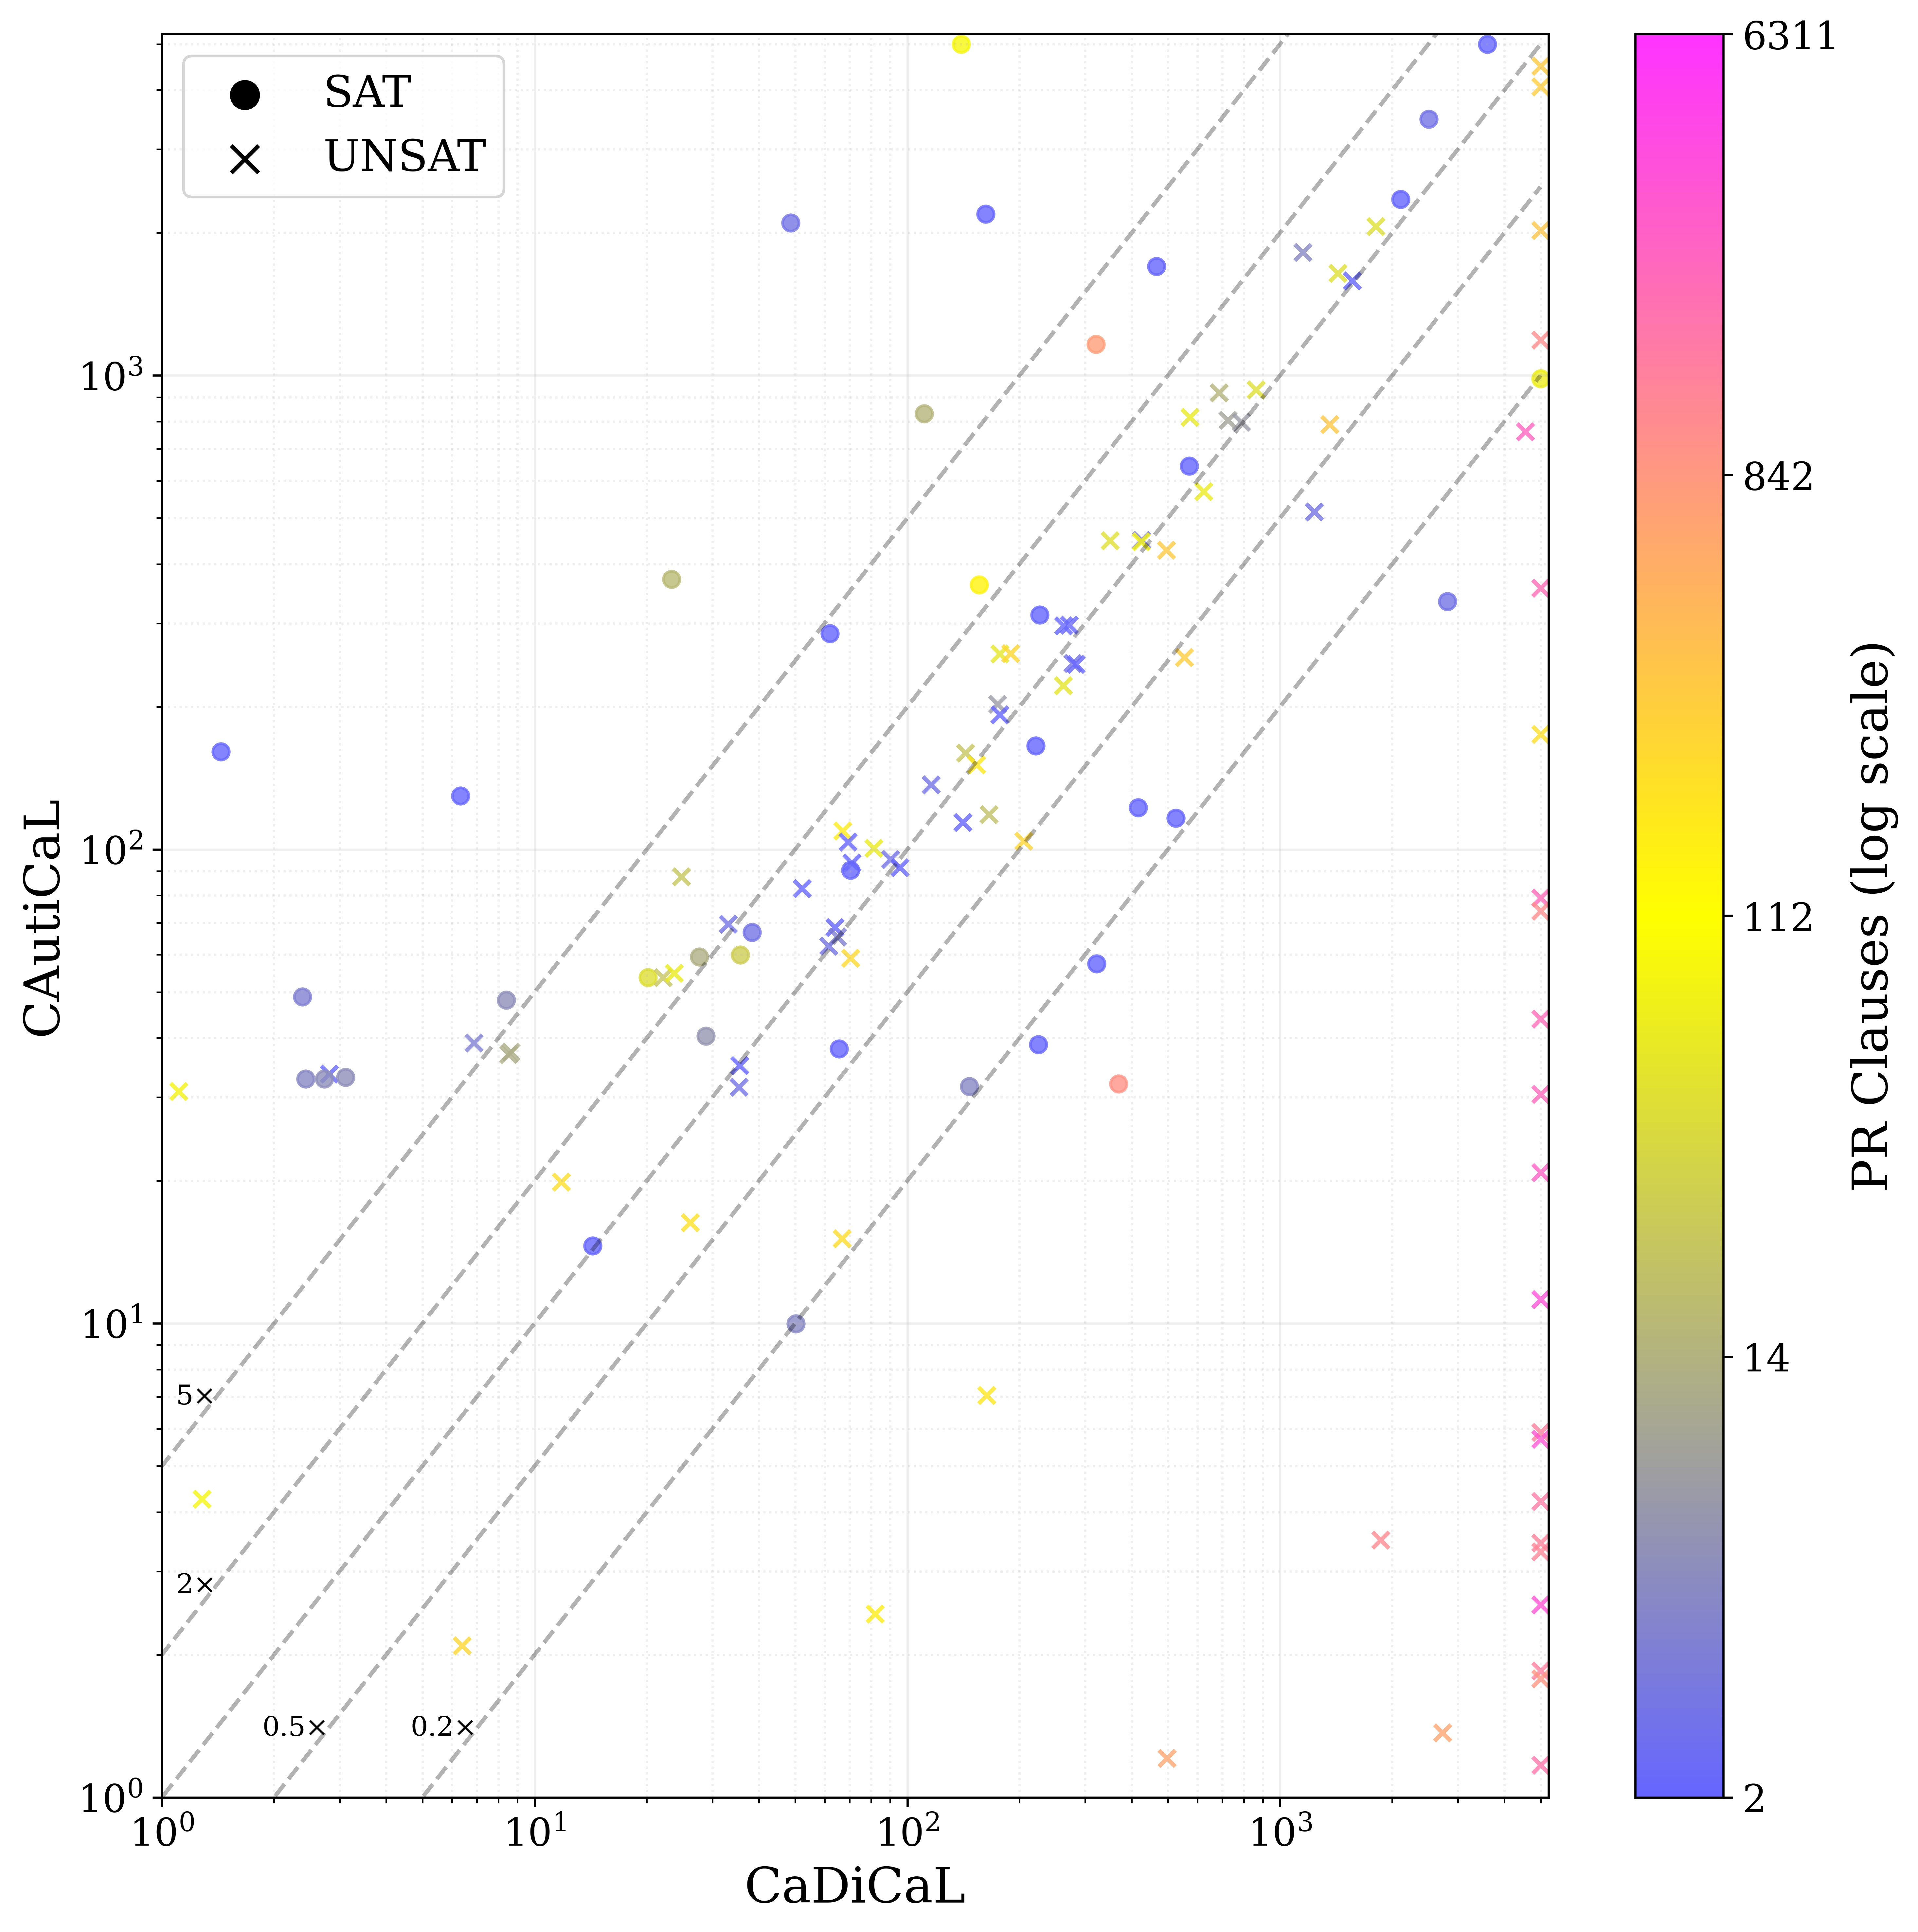
\includegraphics[width=\textwidth]{figs/cadical_vs_cautical_nontrivial.jpg}
        \caption{Comparing \tool to \cadical. The color indicates the number of \pr clauses learnt by \tool}
        \label{fig:cautical-vs-cadical}
    \end{subfigure}
    % \hspace{0.06\textwidth}
    \begin{subfigure}[t]{0.45\textwidth}
        \centering
        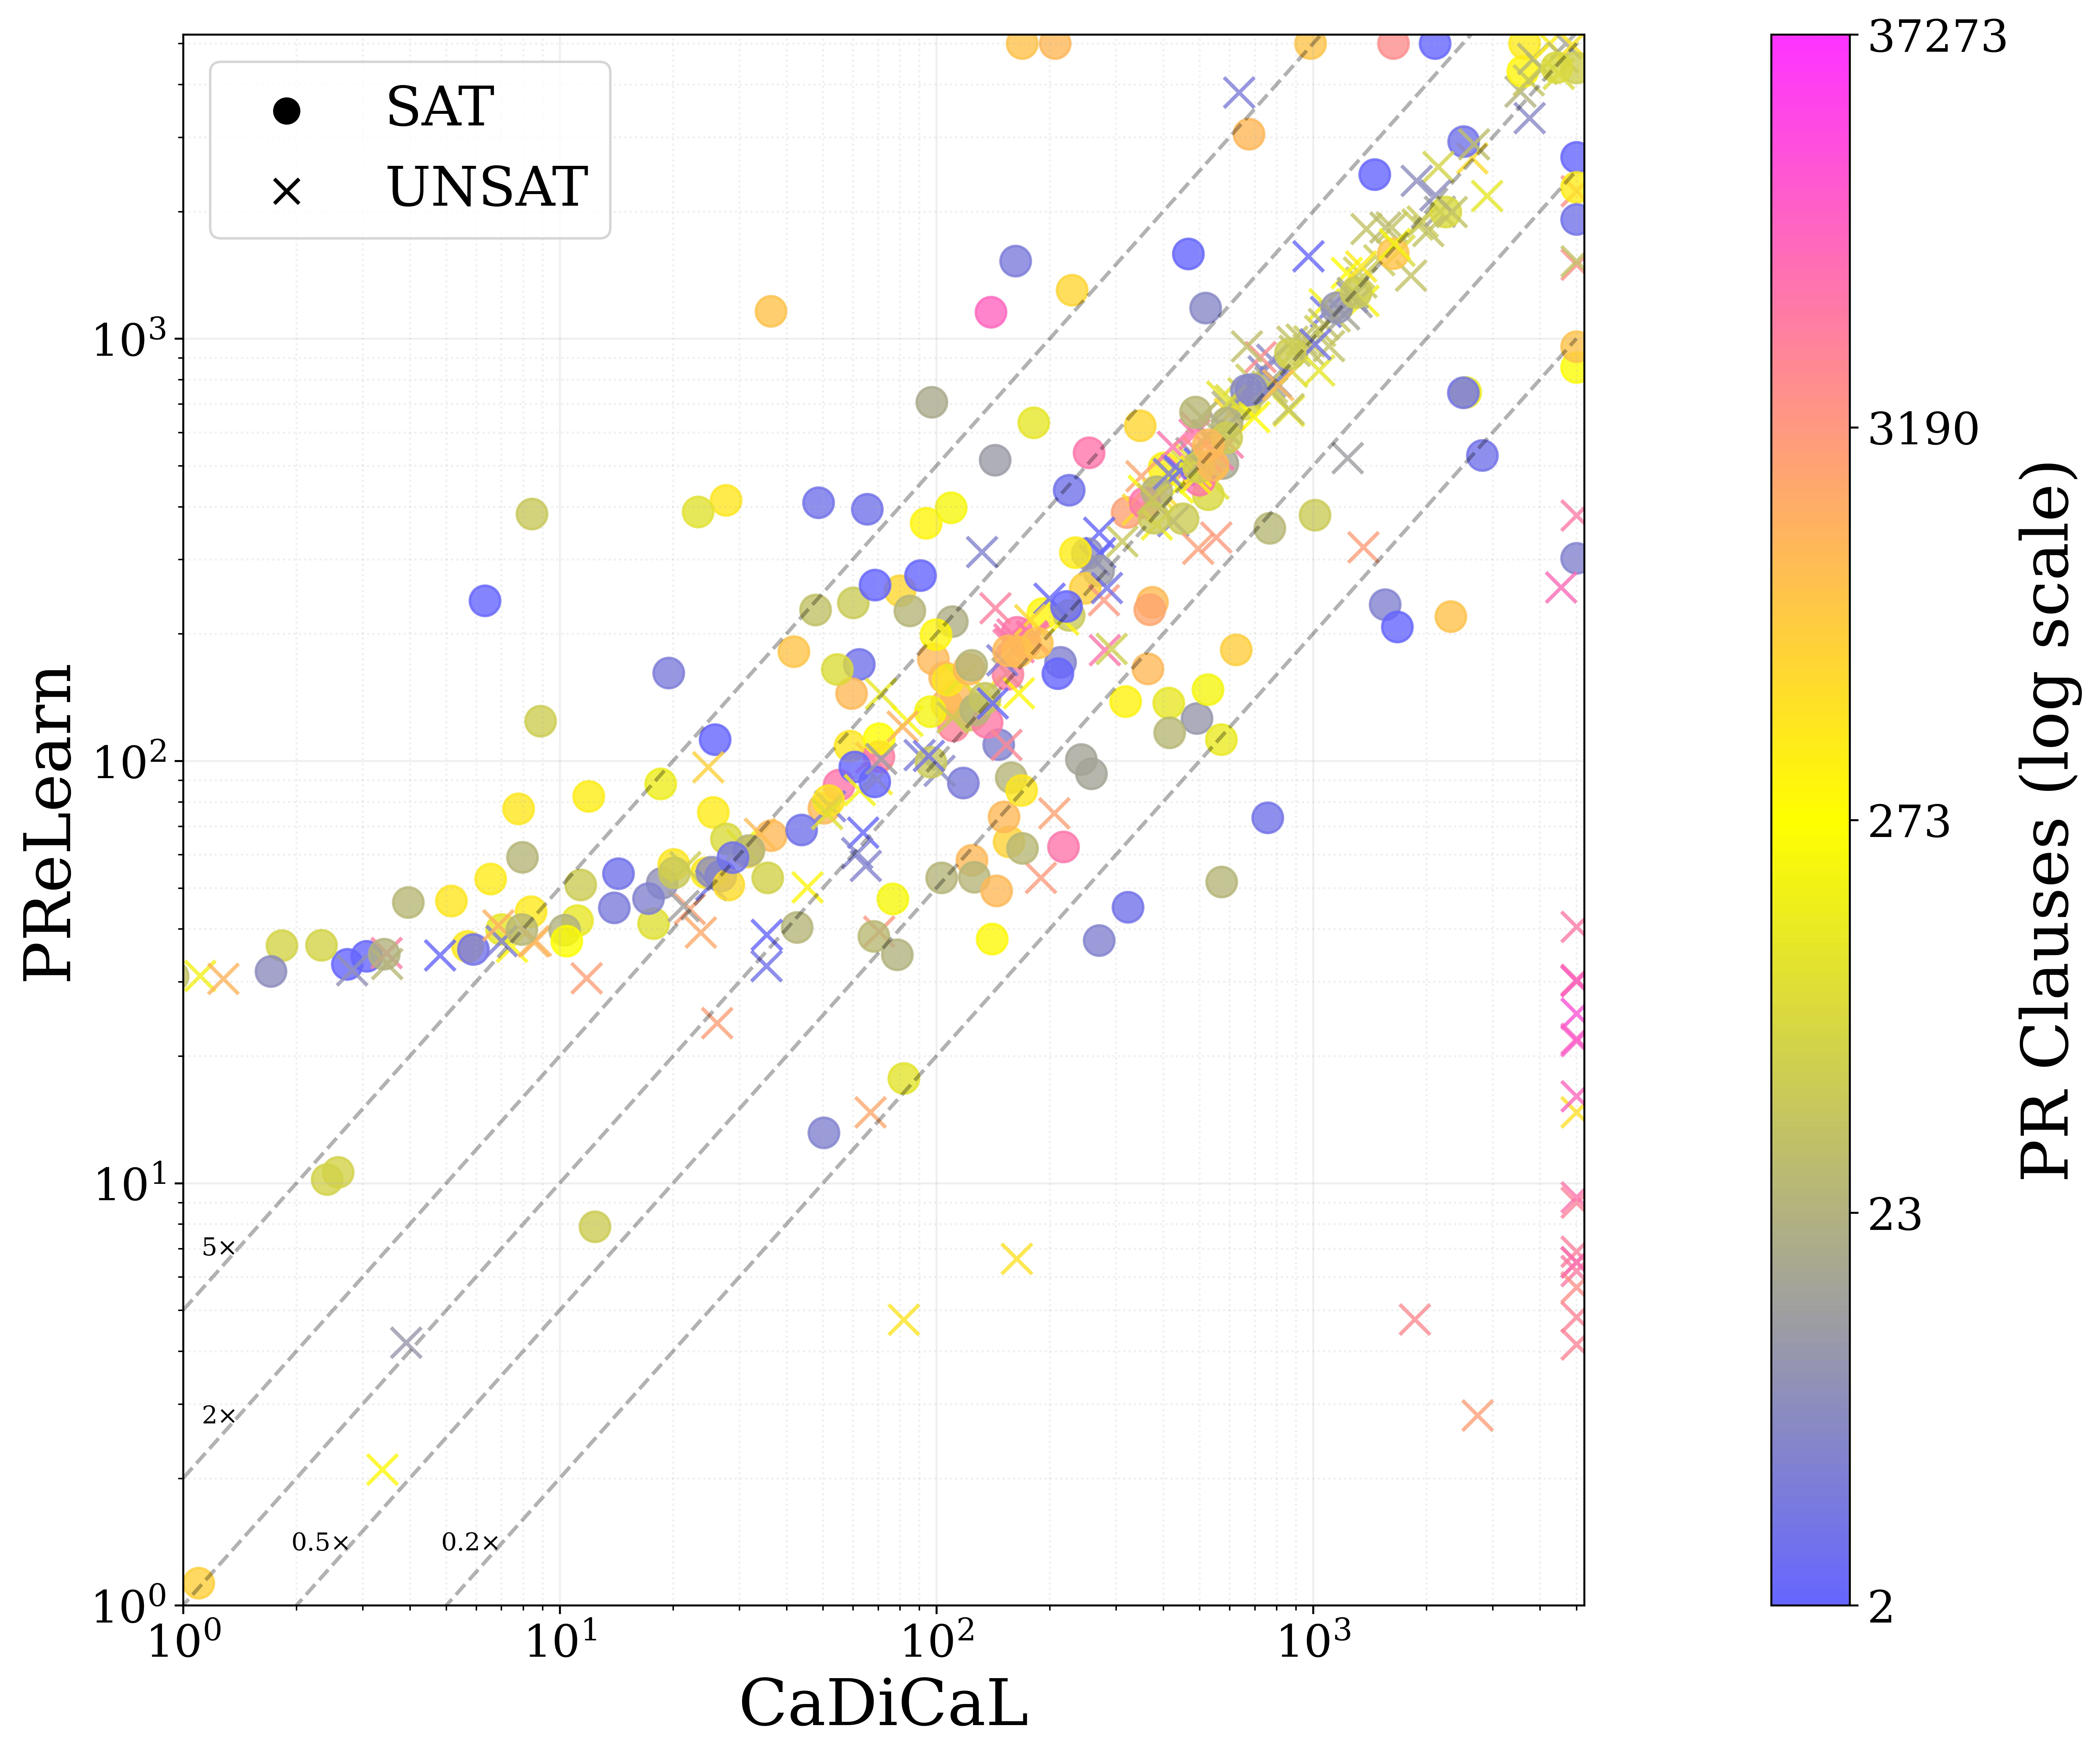
\includegraphics[width=\textwidth]{figs/cadical_vs_prelearn_nontrivial.jpg}
        \caption{Comparing \prelearn to \cadical. The color indicates the number of \pr clauses learnt by \prelearn}
        \label{fig:cautical-vs-prelearn}
    \end{subfigure}
    \caption{Performance comparison of \tool with and \prelearn with \cadical on SAT competition benchmarks. We filter out all benchmarks where the solvers do not learn any \pr clauses. The color indicates the number of \pr clauses learnt by the solver.}
    \label{fig:solver-comparison}
\end{figure*}

We compare the performance of \tool with \cadical and \prelearn on the benchmarks from the '22,'23, and '24 SAT competition's main tracks~\cite{satcomp2022,satcomp2023,satcomp2024}. We remove duplicates and  exclude all benchmarks with more than twenty million clauses. This gives us a total of 1089 benchmarks. We excluded \sadical as it can only solve 22 of these benchmarks.

\autoref{tab:solver-stats} shows the number of instances solved by each solver and the number of queries for which \prelearn and \cadical learn additional \pr clauses, how many improve upon \cadical by at least 5\%, and how many solve a formula that \cadical does not solve. We divide the benchmarks based on number of clauses (0-10k or 10k-20M) and status (SAT or UNSAT).

PAR-2 score is a standard metric used to evaluate the performance of solvers.
It is evaluated as the sum of the runtimes of solved instances and twice the timeout of unsolved instances. On this dataset, \cadical has a PAR2-score of 3521.79 seconds, \prelearn has a PAR2-score of 3331.41 seconds, and \tool has a PAR2-score of 3442.14 seconds. This can be explained by \prelearn solving the most formulae at 771, followed by \tool at 754, and \cadical at 749.

%  I don't know if this actually makes sense
Notably, \tool solves 36 formulae that \cadical does not solve, while \prelearn solves 30 that \cadical does not solve. \tool improves on 219 formulae from \cadical, while \prelearn improves on 146 formulae. We attribute this to more selective \pr clause learning techniques in \tool. Learning unhelpful \pr clauses can have a detrimental effect on performance. \tool only learns 50 \pr clauses or more for 57 formulae, while \prelearn learns 50 \pr clauses or more for 256 formulae. On those clauses, \tool improves the \cadical's runtime by ??\%, while \prelearn improves it by ??\%.

\autoref{fig:solver-comparison} shows \tool and \cadical's performance relative to \cadical. We only include points where \tool (for \autoref{subfig:cautical-vs-cadical}) and \prelearn (for \autoref{subfig:cautical-vs-prelearn}) learn at least one \pr clause. \autoref{subfig:cautical-vs-cadical} shows that \tool learns a large number of \pr clauses for formulae that it can solve quickly and \cadical times out on. \autoref{subfig:cautical-vs-prelearn} shows that \prelearn also solve a number of formulae that \tool cannot, but it learns a large number of \pr clauses for other formulae.







% prelearn PAR score:  3331.406813590451
% cautical PAR score:  3442.137998163452
% cadical PAR score:  3521.7908356290172

\begin{table}[ht]
    \centering
    \sisetup{table-format=3}        % remove if you are not using siunitx
    \begin{tabular}{lrrrrr}
      \toprule
      & \multicolumn{2}{c}{0--10k} & \multicolumn{2}{c}{10k--20M} \\
      \cmidrule(lr){2-3} \cmidrule(lr){4-5}
      & SAT & UNSAT & SAT & UNSAT & Total \\
      \midrule
    %   Total Formulas & 70 & 132 & 395 & 416 & 1099 \\
      \cadical Solved  &  54 &  73 & 319 & 303 & 749 \\
      \midrule
      \prelearn \\
      \; Total &  52 &  90 & 322 & 307 & 771 \\
      \; Learnt clauses   &  40 &  73 & 179 & 145 & 431\\
      \; Learnt $>50$ clauses   &  22 &  51 & 104 &  79 & 256\\
      \; Improved &  11 &  42 &  57 &  36 & 146\\
      \; Exclusively &   1 &  17 &   6 &   6 & 30 \\
      \midrule
      \tool \\
      \; Total &  52 &  87 & 317 & 298 & 754 \\
      \; Learnt clauses     &   16 &  58 &  30 &  35 & 139 \\
      \; Learnt $>50$ clauses  &   1  &  39 &  6 &  11 & 57 \\
      \; Improved &  23  &  48 &  89 &  59 & 219 \\
      \; Exclusively &   0 &  18 &   9 &   9 & 36 \\
      \bottomrule
    \end{tabular}
    \caption{Number of solved instances.}
    \label{tab:solver-stats}
  \end{table}

  % Category                  0-10k SAT  0-10k UNSAT  10k-20M SAT  10k-20M UNSAT  20M+ SAT  20M+ UNSAT  Total
% Total Formulas                   70          132          395            416        40          46   1099 -> issue with this total is that certain formula statuses are unknown, so not counted here
% Cadical Solved                   54           73          319            303        35          46    830
% Has PR Clauses                   40           73          179            145         0           3    440
% Has Many PR Clauses              22           51          104             79         0           0    256
% Prelearn Solved                  52           90          322            307        35          46    852
% Prelearn Only                     1           17            6              6         0           0     30
% Prelearn Improved                11           42           57             36         1           1    148
% Cautical Solved                  52           87          317            298        32          29    815
% Cautical Only                     0           18            9              9         0           0     36
% Cautical Improved                23           48           89             59         0           8    227
% Blocked Clauses                  16           58           30             35         0           0    139
% Has Many Blocked Clauses          1           39            6             11         0           0     57



  \begin{figure*}[!t]
    \centering
    \begin{subfigure}[t]{0.45\textwidth}
        \centering
        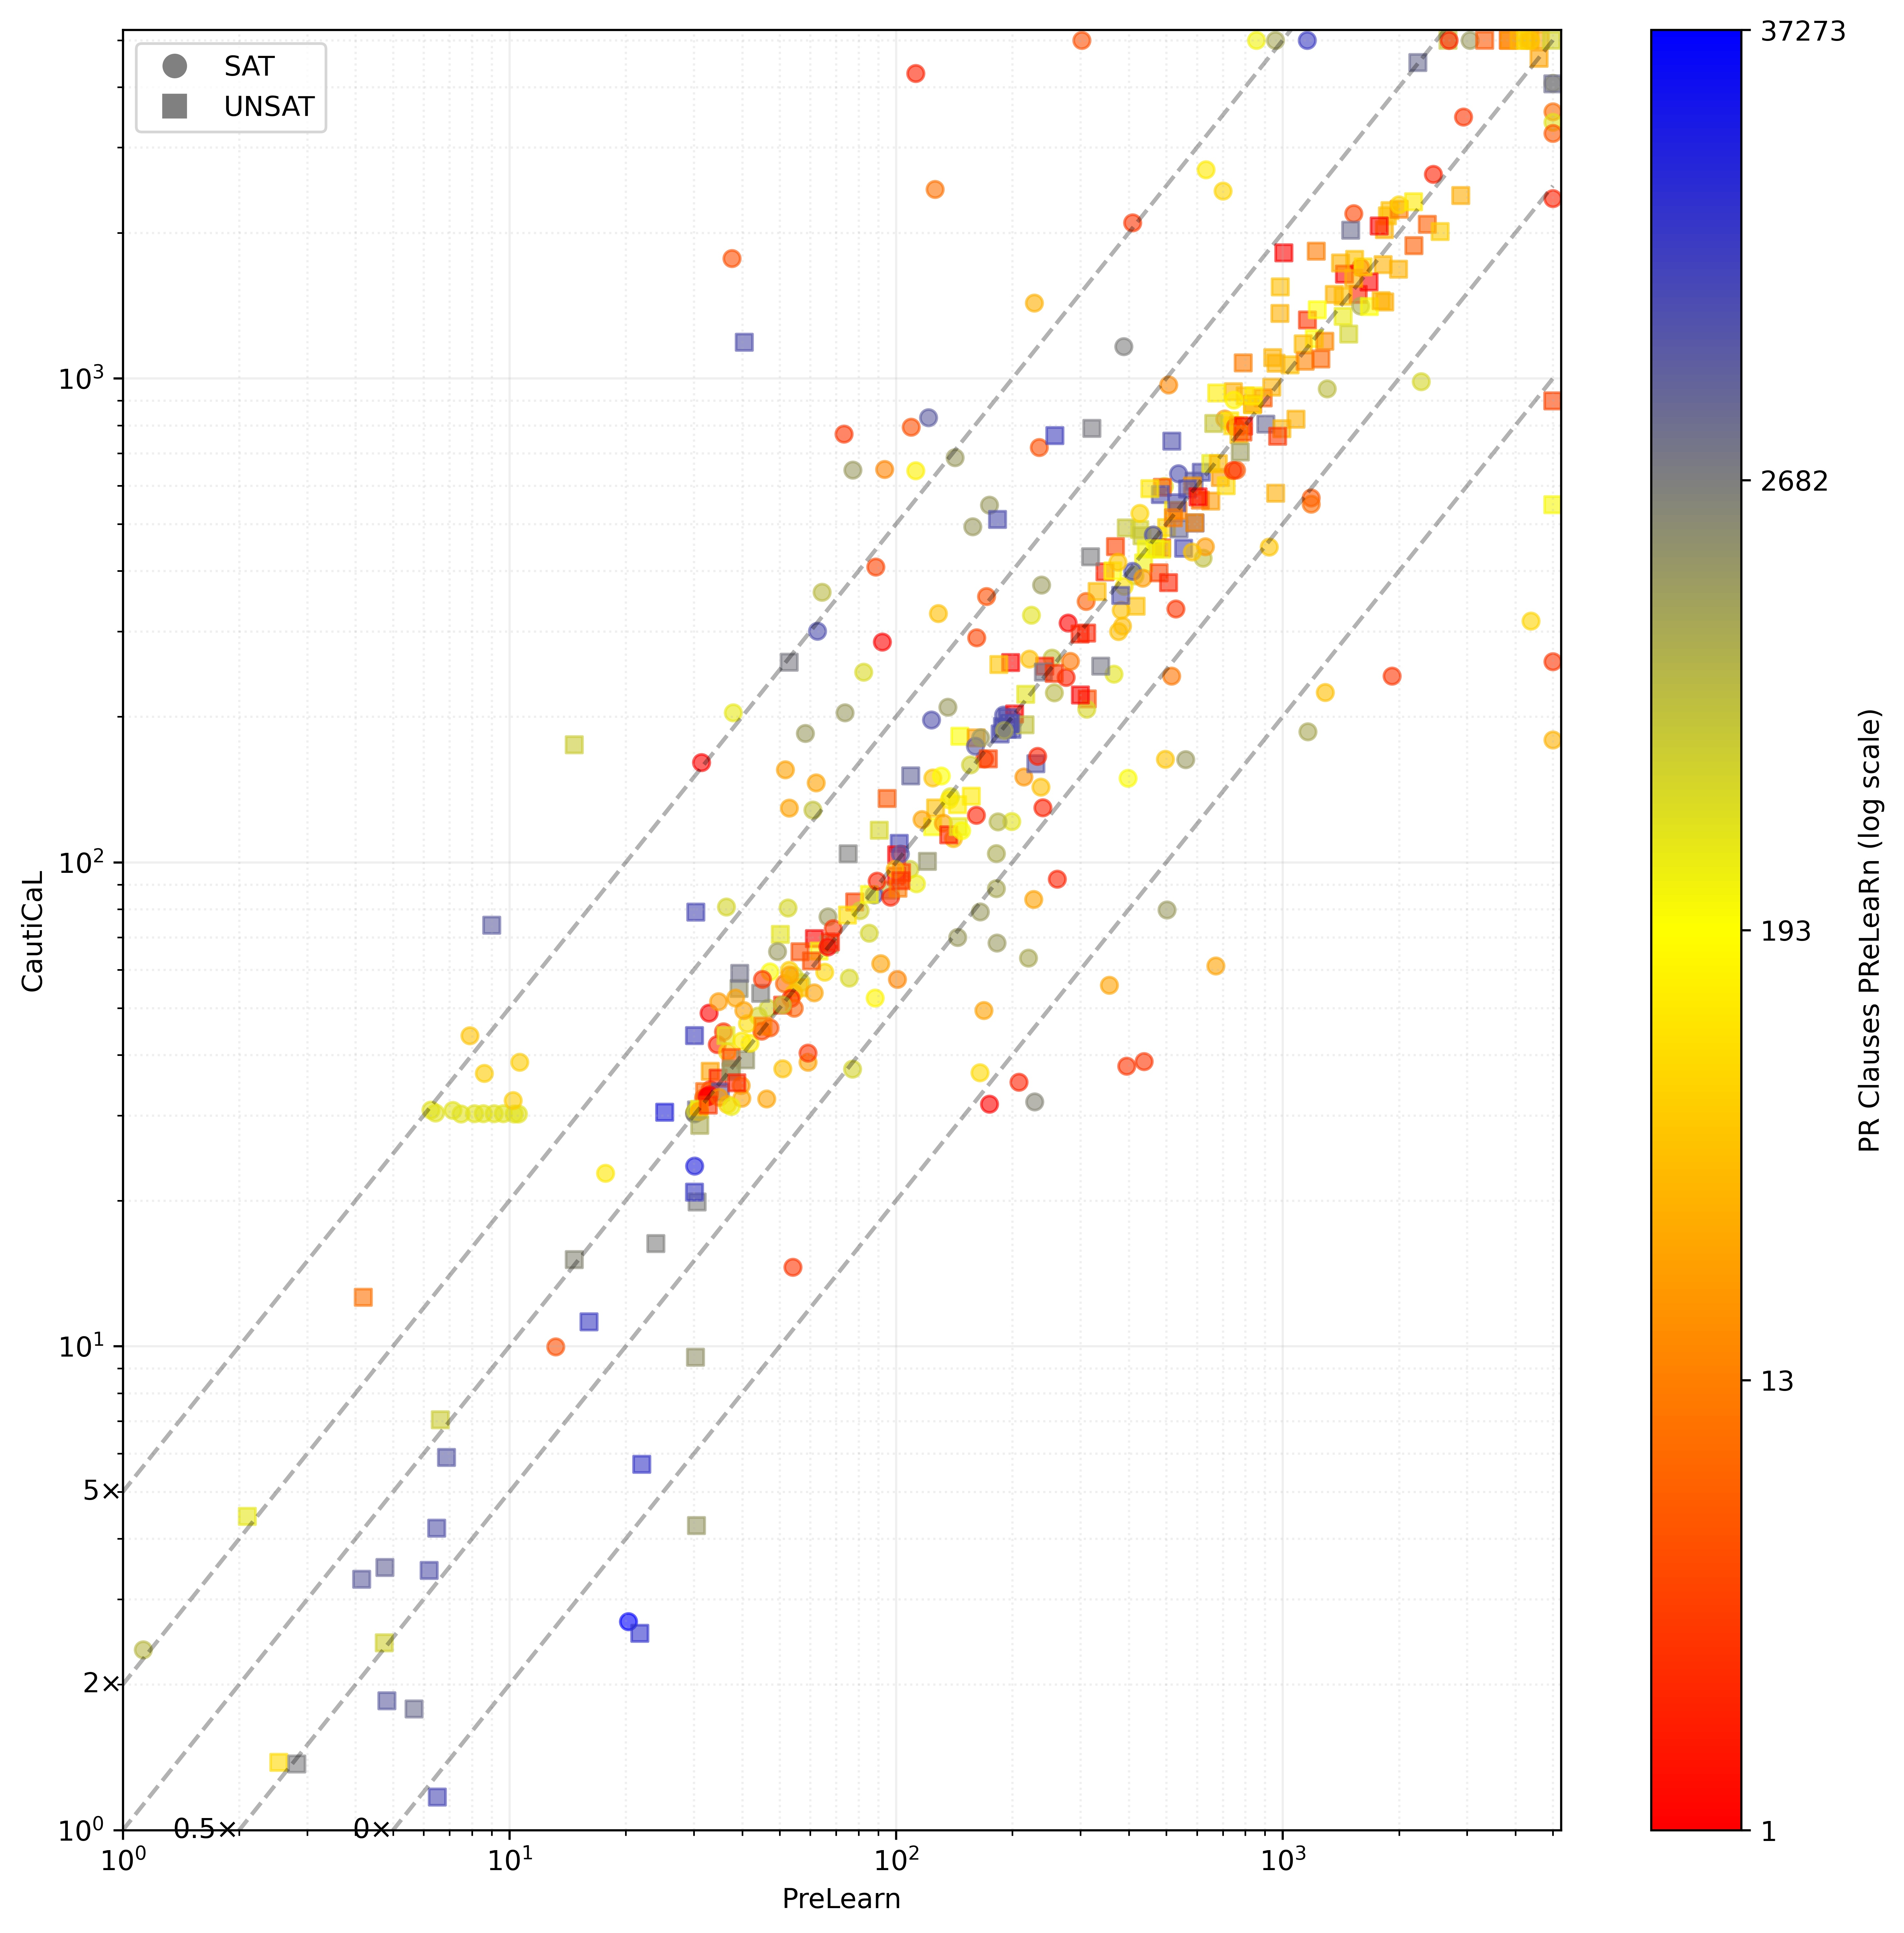
\includegraphics[width=\textwidth]{figs/prelearn_vs_cautical.jpg}
        \subcaption{Performance comparison of \tool to \prelearn. The color indicates the number of \pr clauses learnt by \tool. We filter out all formula where neither \tool nor \prelearn learnt any \pr clauses.}
        \label{fig:cautical-vs-cadical}
    \end{subfigure}
    % \hspace{0.06\textwidth}
    \begin{subfigure}[t]{0.45\textwidth}
        \centering
        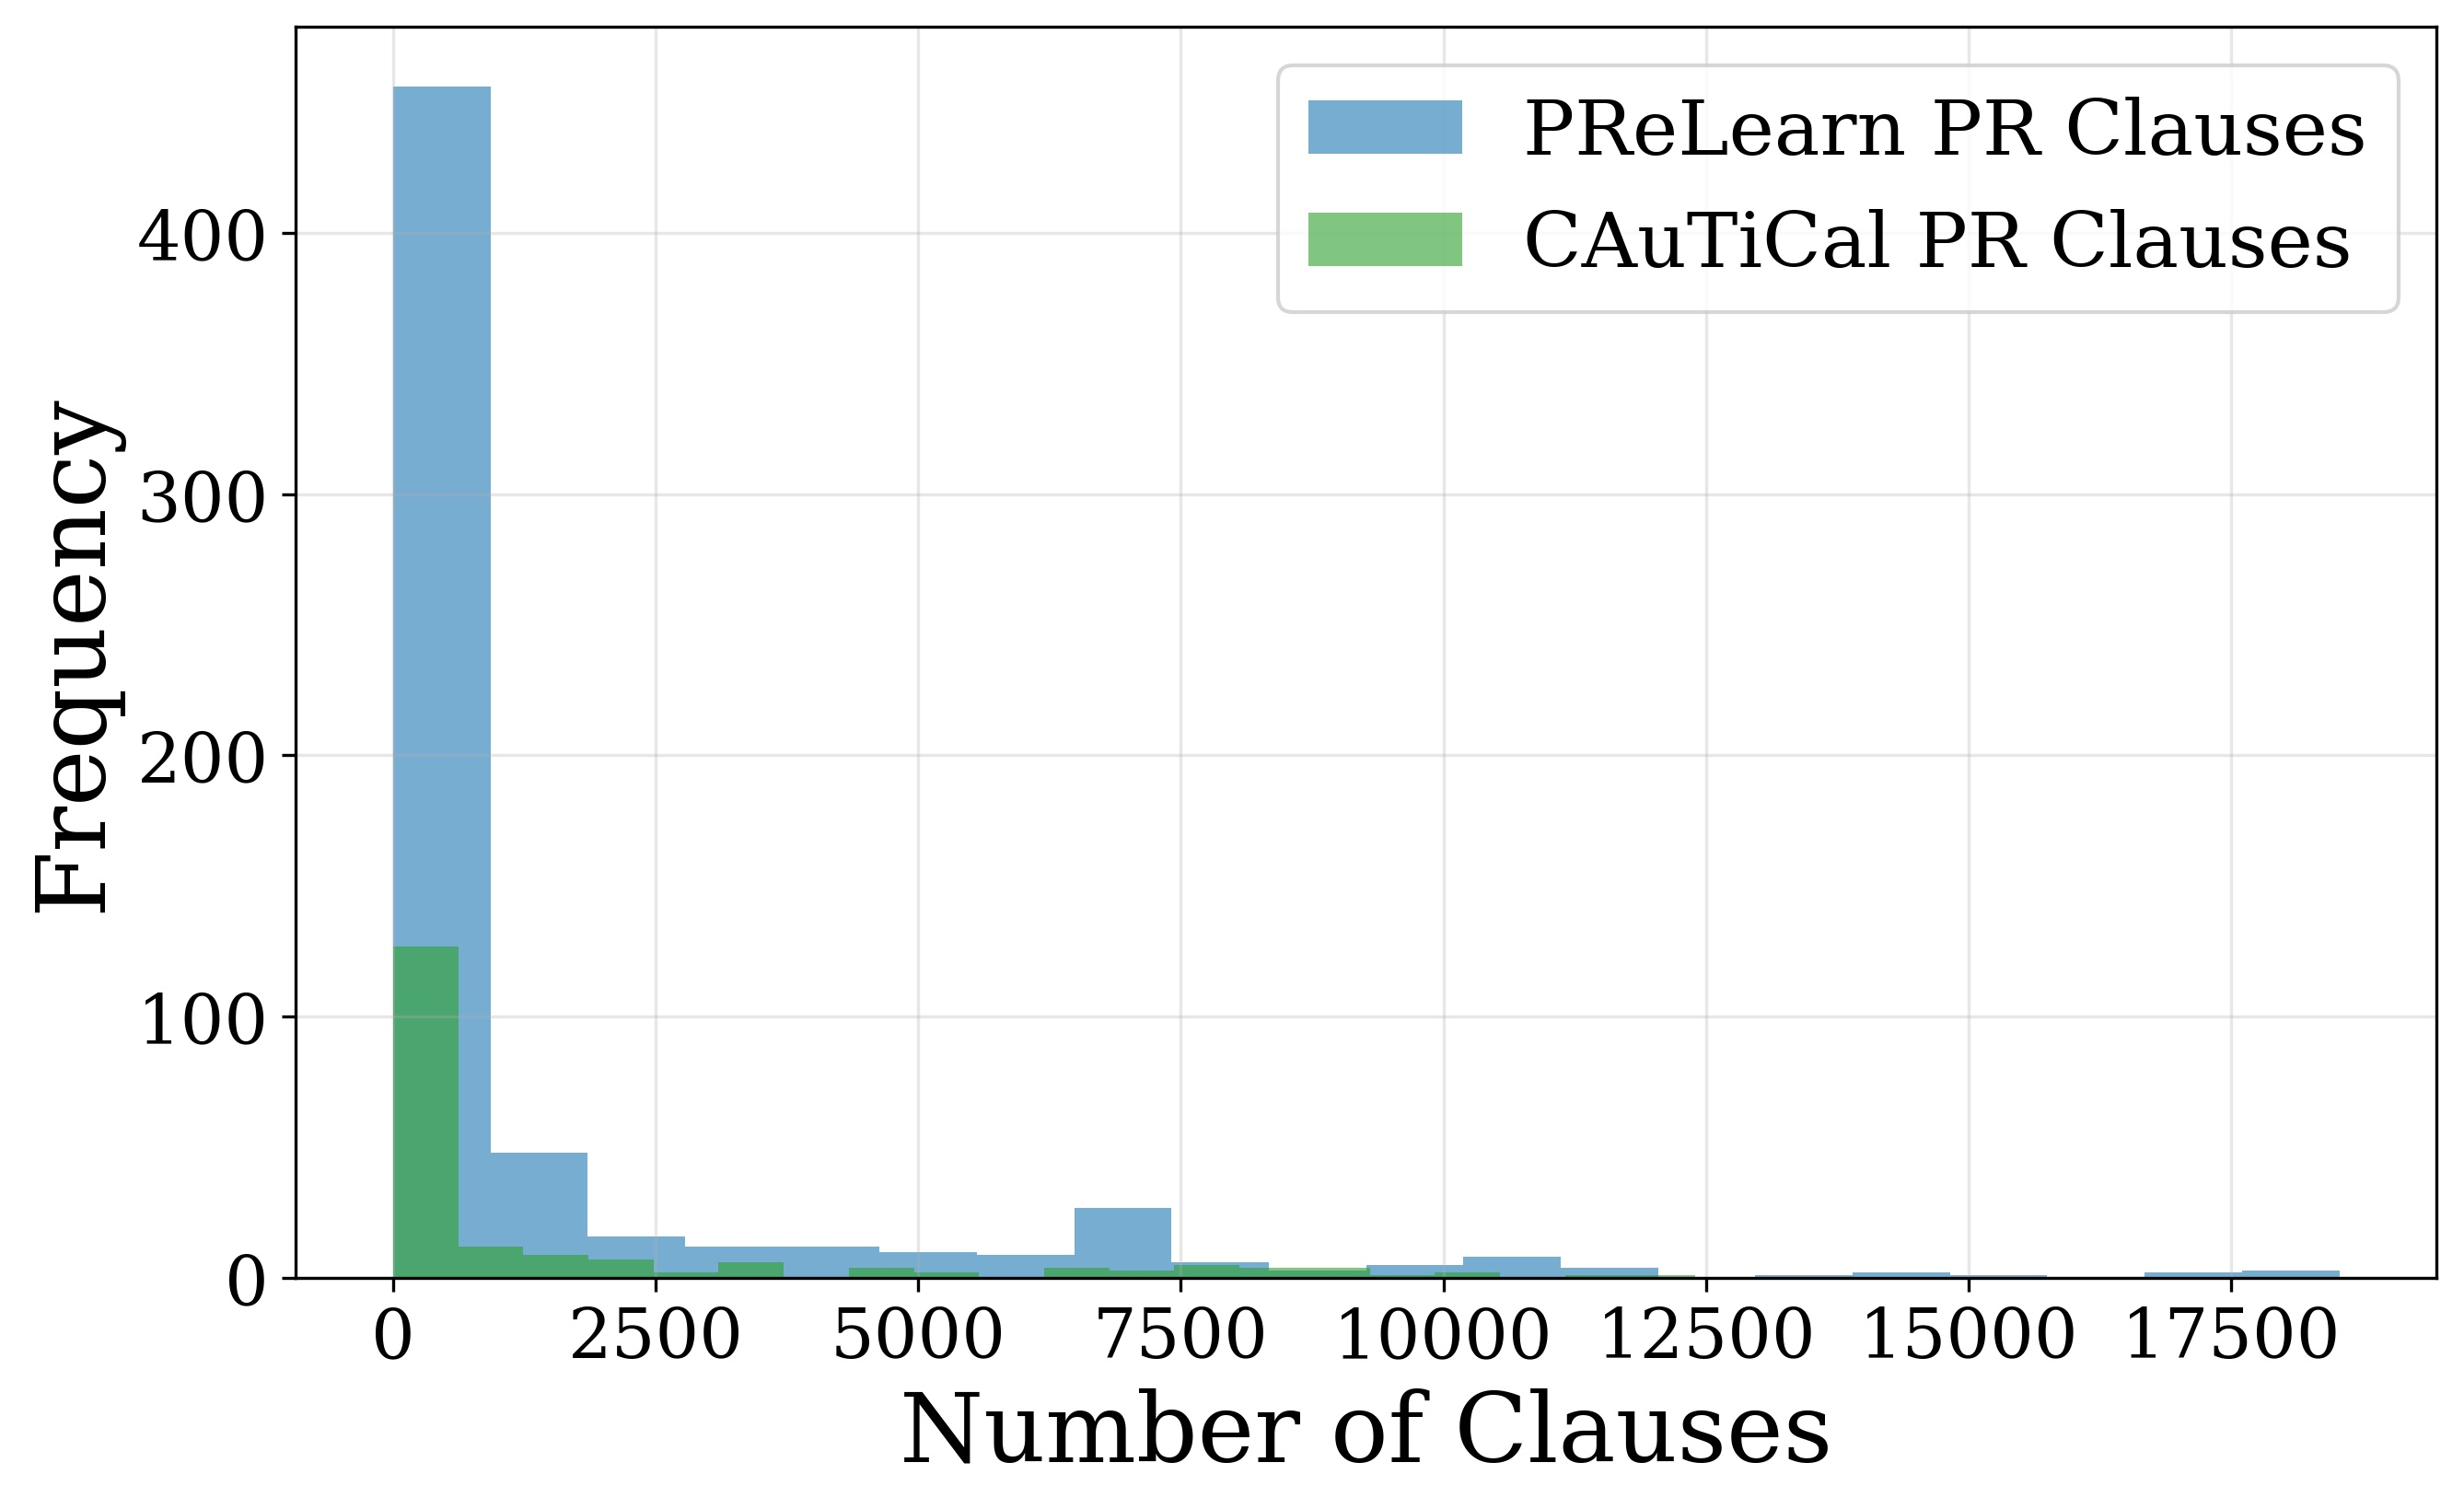
\includegraphics[width=\textwidth]{figs/clauses_histogram.jpg}
        \subcaption{Histogram showing the number of \pr clauses learnt by \tool and \prelearn}
        \label{fig:cautical-vs-prelearn}
    \end{subfigure}
    \caption{Comparison of \tool and \prelearn on SAT competition benchmarks.}
    % \label{fig:solver-comparison}
\end{figure*}





% \subsection{\toolminus}

% Motivated by the fact that \tool improves mostly on formulae where it learns many clauses, we define a new variant \toolminus. After running the 30 second preprocessing step, if \toolminus does not learn at least $50$ \pr clauses, it will completely reset the context and run cadical. In \autoref{fig:toolminus-comparison}, we compare \tool to \prelearn and \toolminus to \prelearn on the SAT competition benchmarks.


% \begin{figure*}[!t]
%     \centering
%     \begin{subfigure}[t]{0.45\textwidth}
%         \centering
%         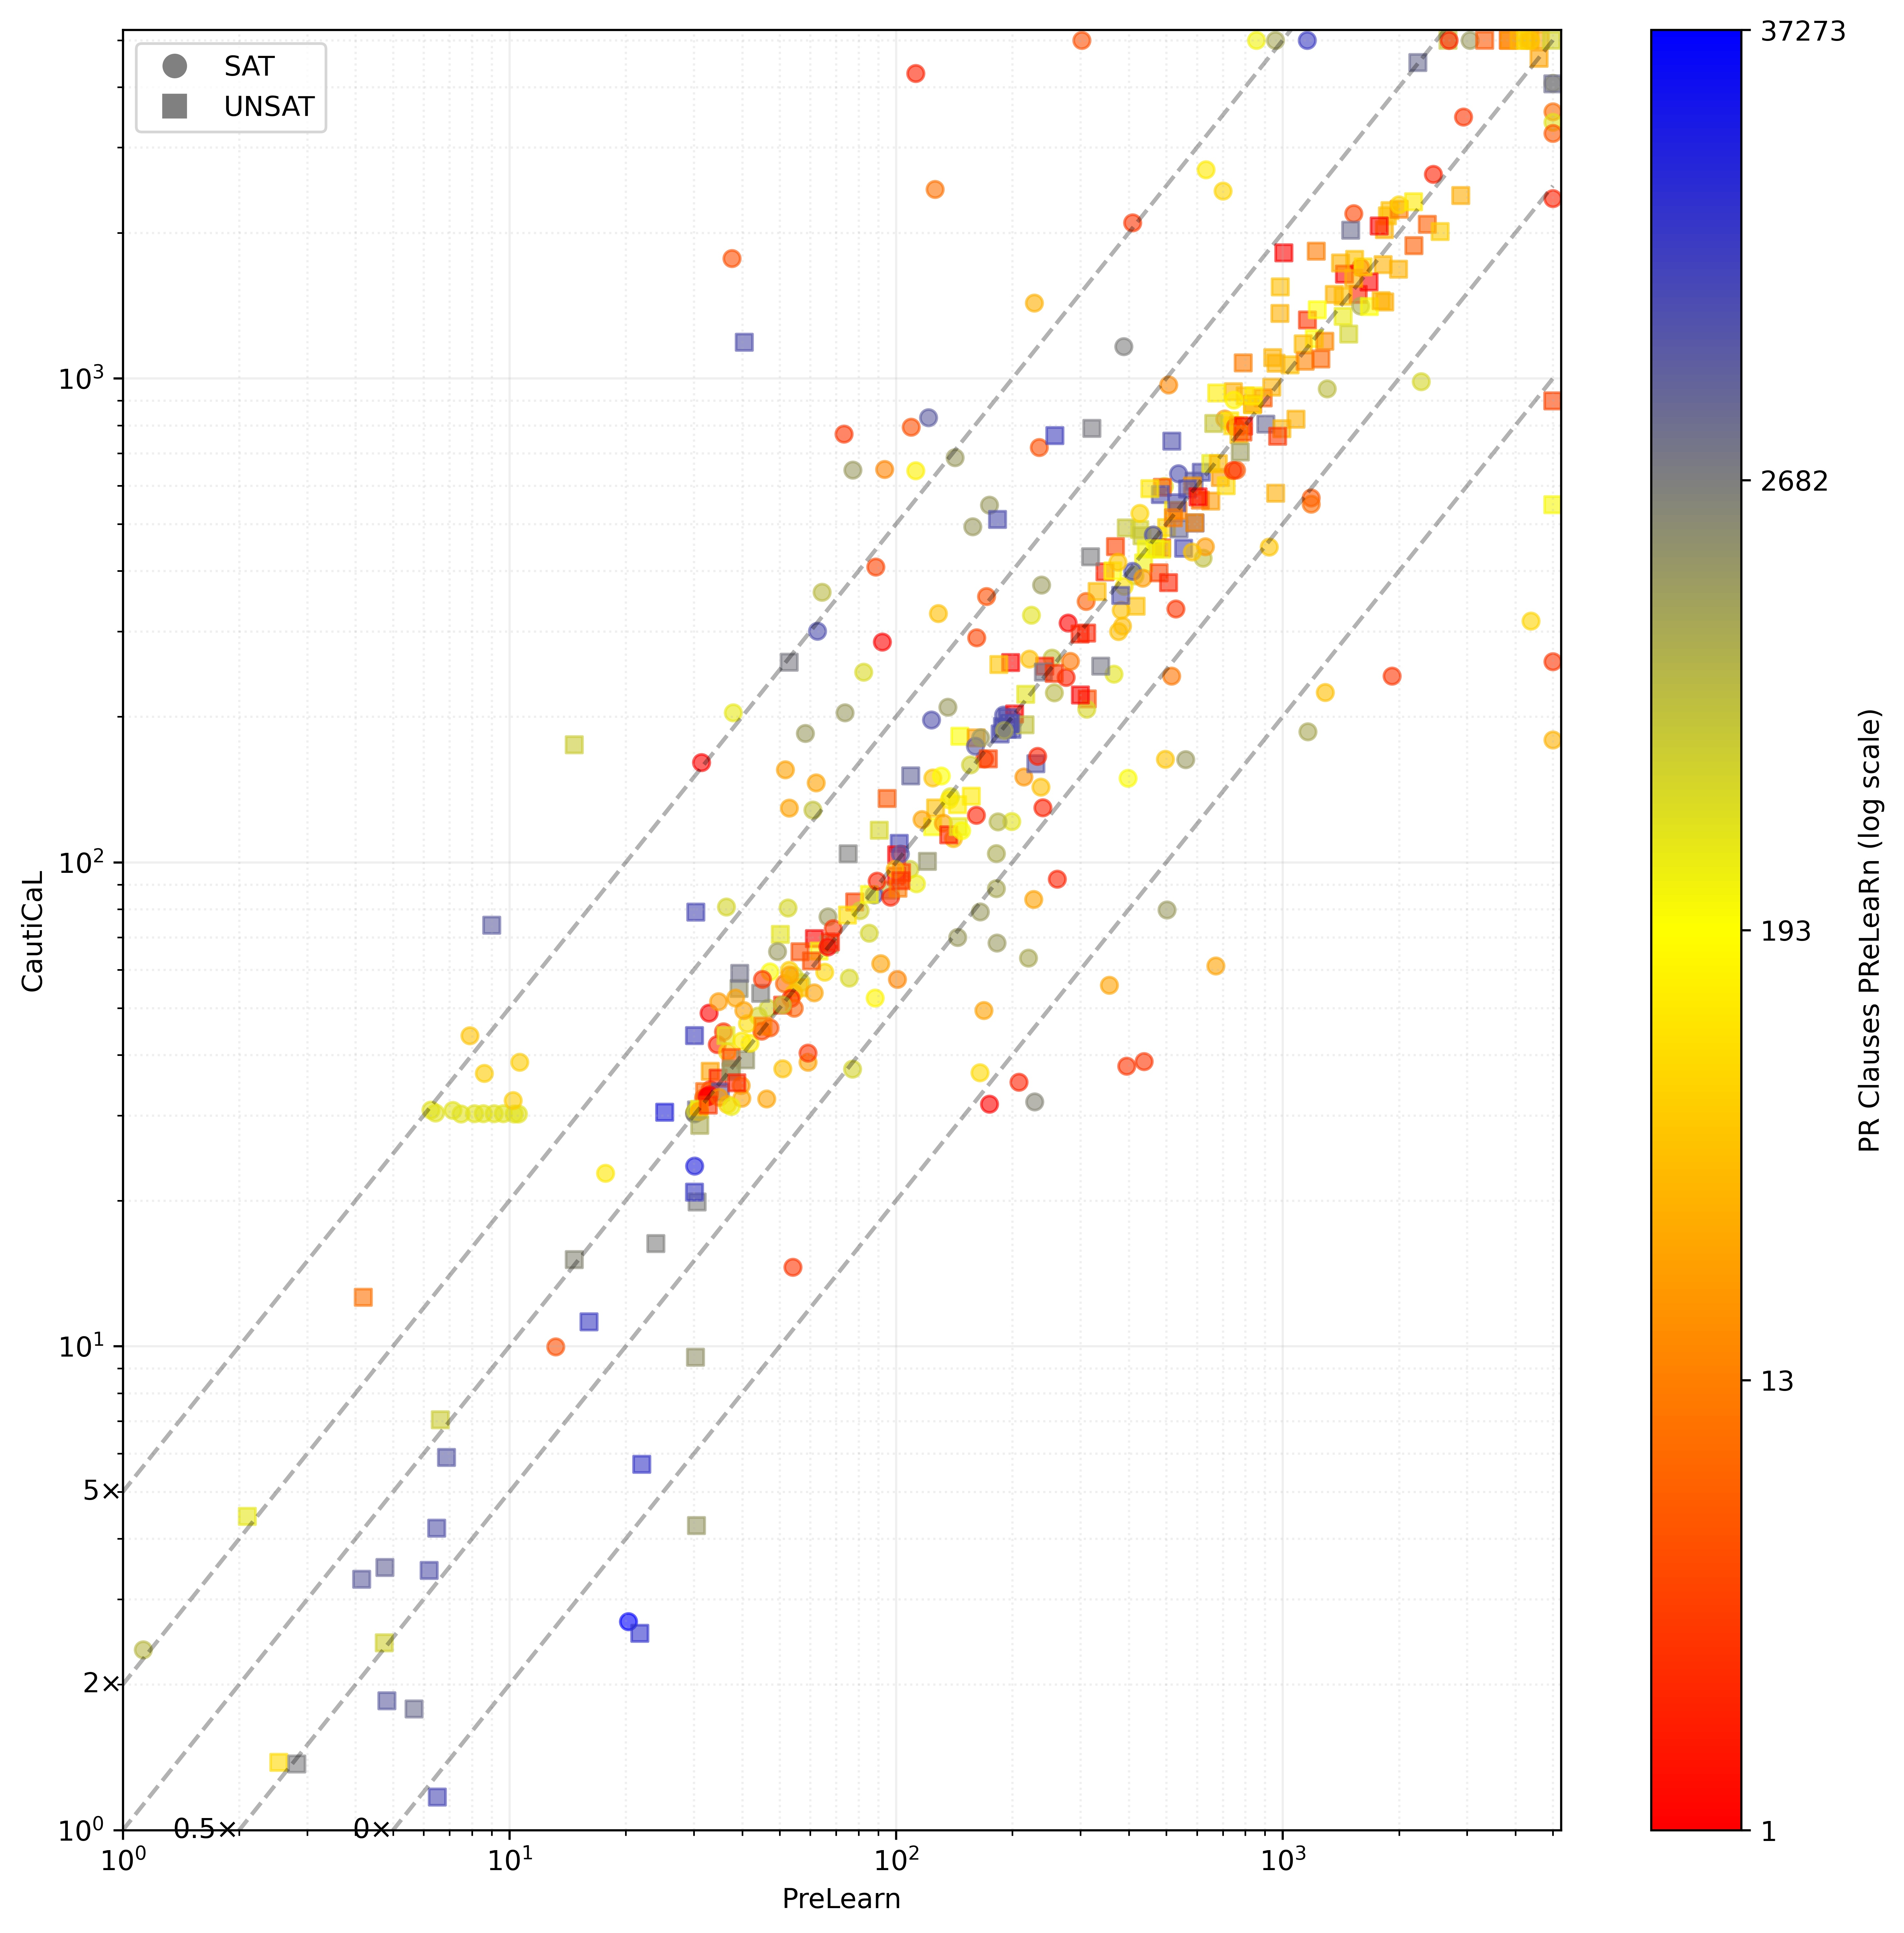
\includegraphics[width=\textwidth]{figs/prelearn_vs_cautical.jpg}
%         \caption{Comparing \tool to \prelearn. The color indicates the number of \pr clauses learnt by \tool}
%         \label{fig:cautical-vs-cadical}
%     \end{subfigure}
%     % \hspace{0.06\textwidth}
%     \begin{subfigure}[t]{0.45\textwidth}
%         \centering
%         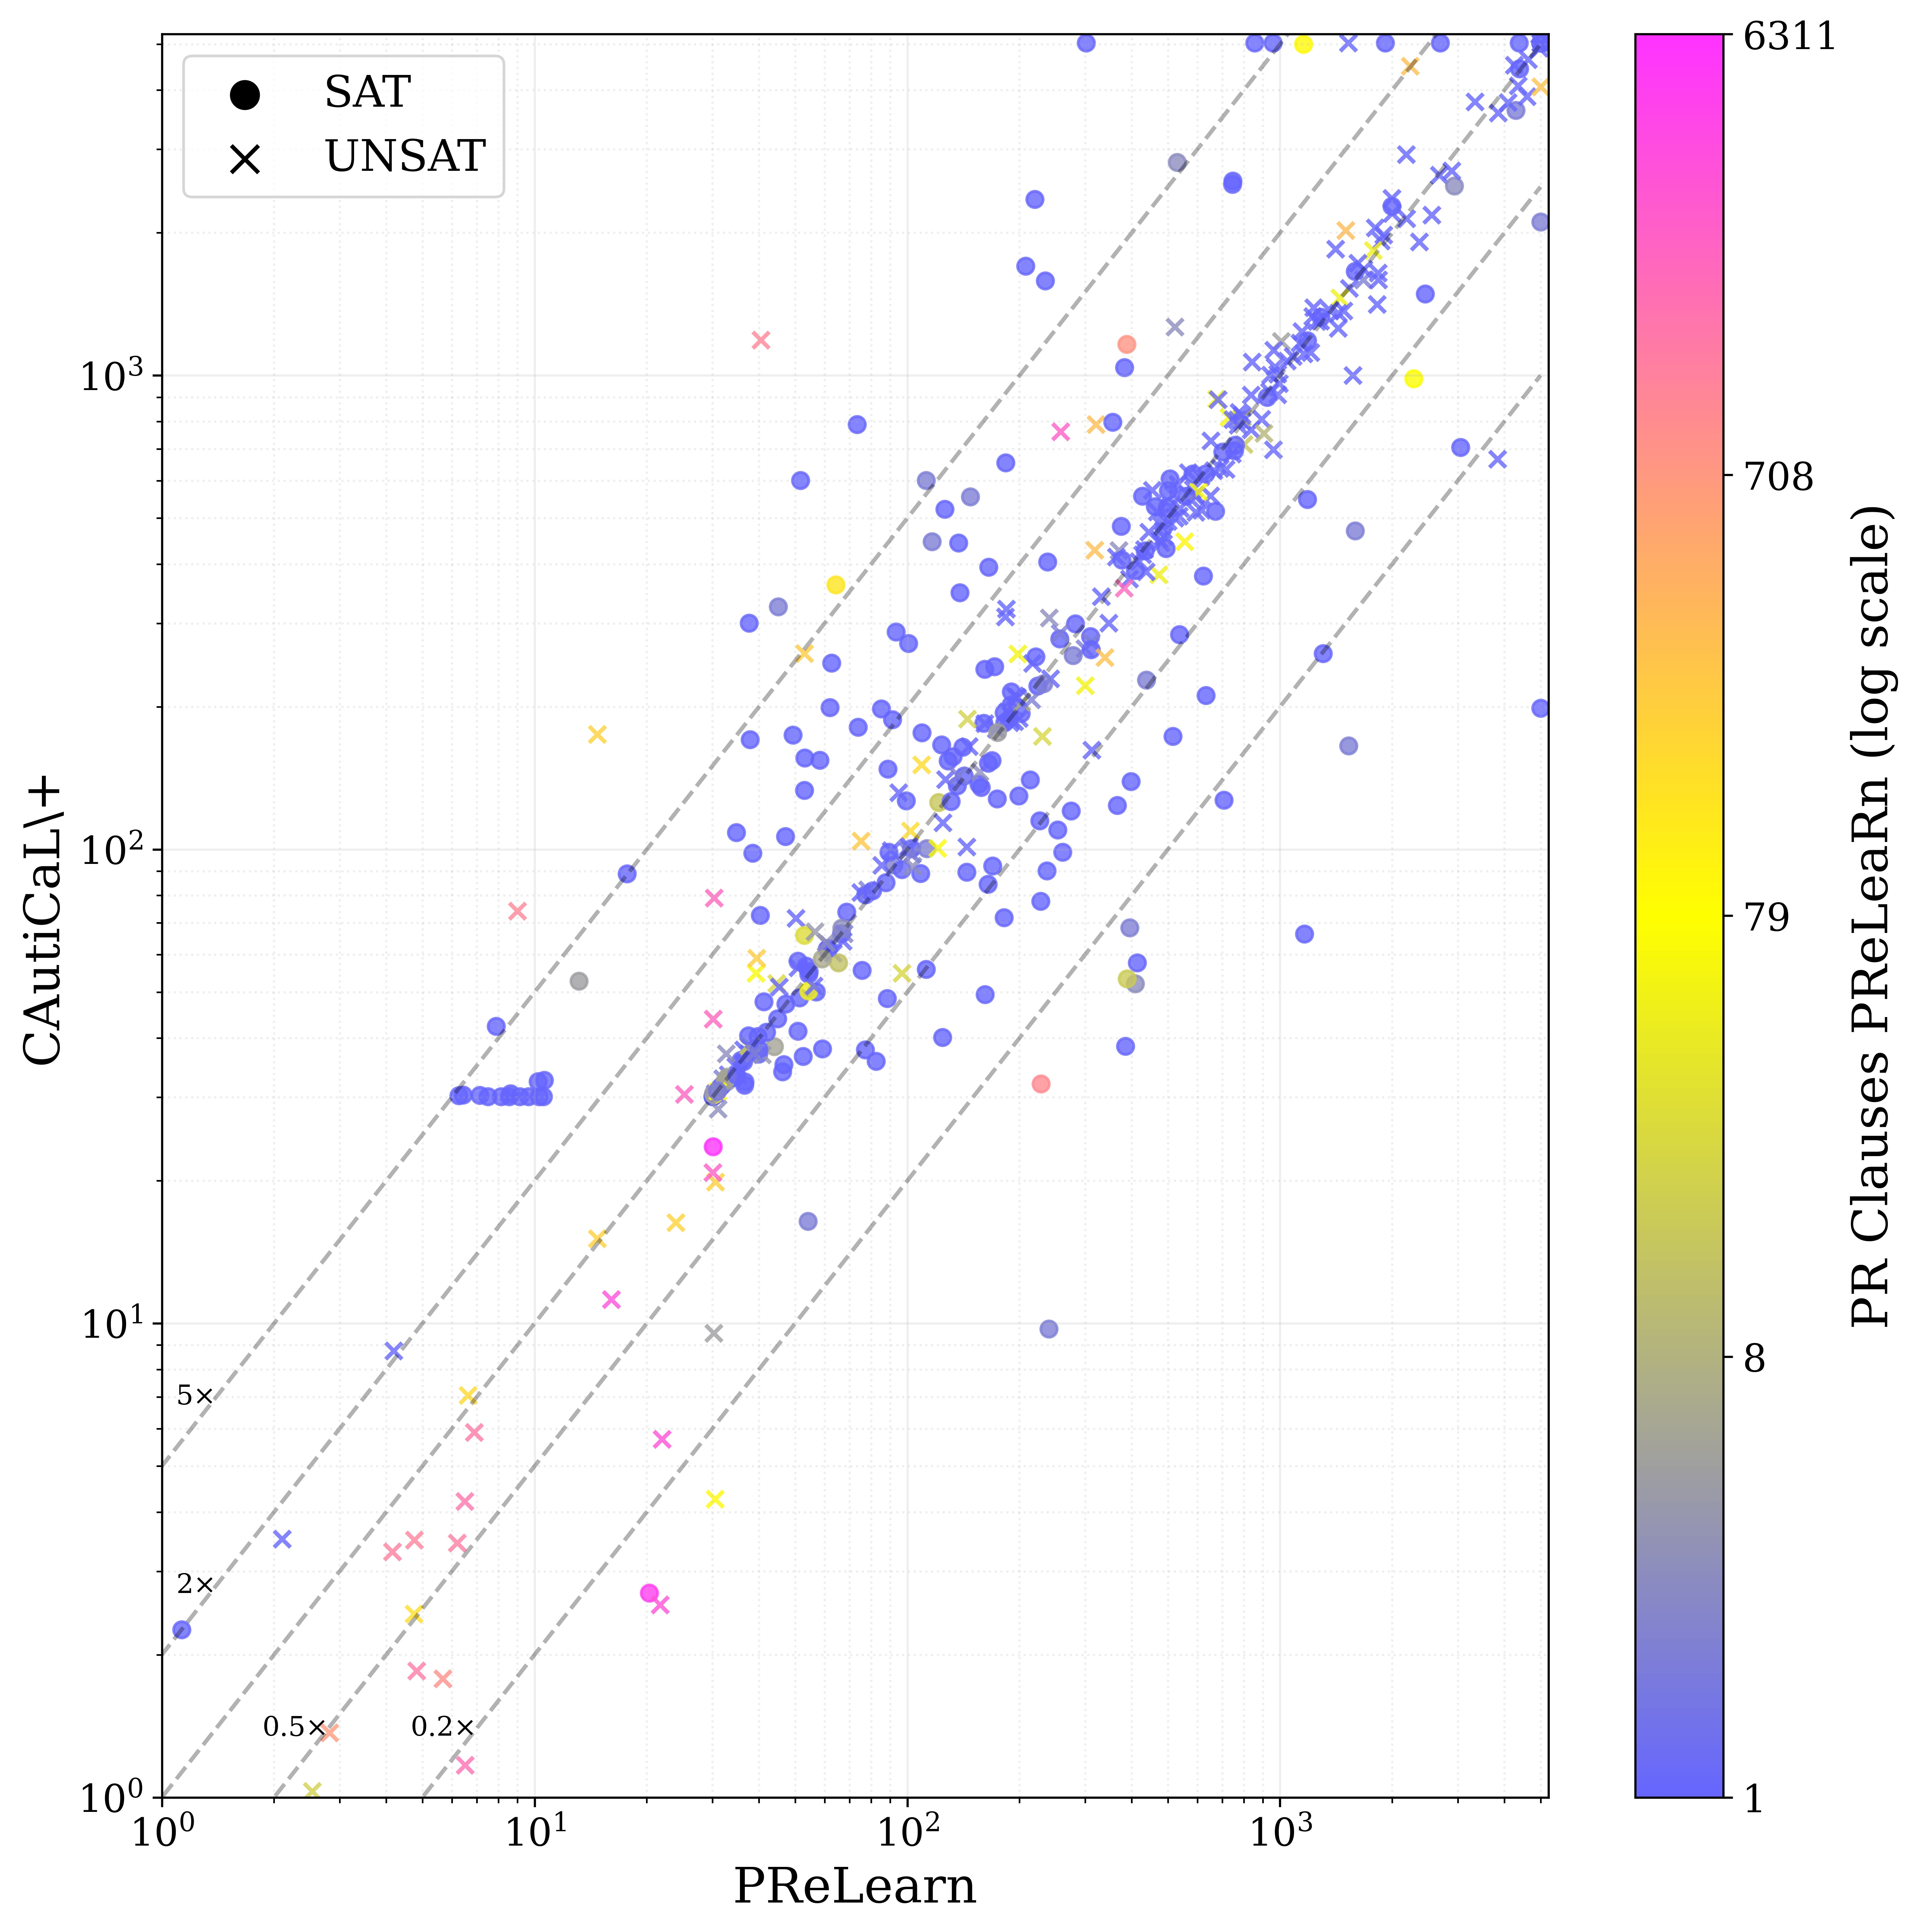
\includegraphics[width=\textwidth]{figs/prelearn_vs_cautical_minus_time.jpg}
%         \caption{Comparing \toolminus to \prelearn. The color indicates the number of \pr clauses learnt by \toolminus}
%         \label{fig:cautical-vs-prelearn}
%     \end{subfigure}
%     \caption{Performance comparison of \tool with and \toolminus with \prelearn on SAT competition benchmarks. We filter out all benchmarks where both \tool and \prelearn do not learn any \pr clauses. The color indicates the number of \pr clauses learnt by the \tool or \toolminus.}
%     % \label{fig:solver-comparison}
% \end{figure*}

% version of the graphs without filtering out clauses:
% prelearn_vs_cautical.jpg


\subsection{Discussion of Benchmark Families}~\label{subsec:eval-discussion}

We identify six benchmark families for which \pr clauses perform well. We choose them  based on prior work ~\cite{prelearn} and our experiments on SAT competition benchmarks:

\begin{enumerate}
    \item \texttt{mutilated-chessboard}: A famous problem asking if one can use $2$-by-$1$ tiles to cover an $n$-by-$n$ chessboard with opposite corners removed. This is known to be difficult for resolution~\cite{chessboard-resolution}, but have $O(n^3)$ \pr proofs~\cite{mutilatedchessboard-pr}.
    \item \texttt{perfect-matching}: A generalization of the pigeonhole principle and mutilated chessboard problems with various at-most-one constraints~\cite{bipartgen}
    \item \texttt{pcmax-scheduling}: A problem encoding the scheduling problem mapping $n$ tasks with known execution times to $m$ identical processors~\cite{pcmax}.
    % \item https://helda.helsinki.fi/server/api/core/bitstreams/3f1f286b-3def-49e9-98ba-f887b1bc250e/content -> page 31
    \item \texttt{register-allocation}: A problem representing the graph coloring problem generated by simulating register allocation on individual Python functions~\cite{register-allocation}.
    \item \texttt{relativized\_pigeonhole}: A generalization of the pigeonhole principle where we place $n+1$ pigeons in $n$ holes with $k$ nesting places~\cite{relativized-pigeonhole}.
    % todo: ask joseph about citation
    \item \texttt{satcoin}: An unsatisfiable variant of a bitcoin mining problem~\cite{satcoin}.
    \item \texttt{test=configuration}: A problem asking if there is a list of configurations of size $k$ that covers every pairwise combination of configurations of a SAT solver~\cite{test-configuration}.
\end{enumerate}

These formulas are mostly UNSAT as these are most benefitted by \pr clause learning. SAT formulas are very sensitive to search heuristics, so adding a \pr clause can have a significant (positive or negative) effect on performance, regardless if a clause is actually useful. \autoref{fig:solver-comparison-familis} compares the performance of \tool compared to \cadical and \prelearn on the benchmark families. 

\tool compares favorably to \cadical on all benchmark families (except \texttt{relativized\_pigeon\_hole}), showing especially large speedups on \texttt{register\_allocation}, \texttt{mutilated-chessboard} and \texttt{perfect-matching}.
\prelearn overall performs better with large speedups over \tool on \texttt{test-configuration} and \texttt{pcmax-scheduling}. \tool performs better on smaller instances of \texttt{register-allocation} and \texttt{mutilated-chessboard}, while \prelearn performs better on larger instances. \tool can also solve a few instances of \texttt{satcoin} that \prelearn cannot.


\begin{figure*}[!t]
    \centering
    \begin{subfigure}[t]{0.45\textwidth}
            \centering
            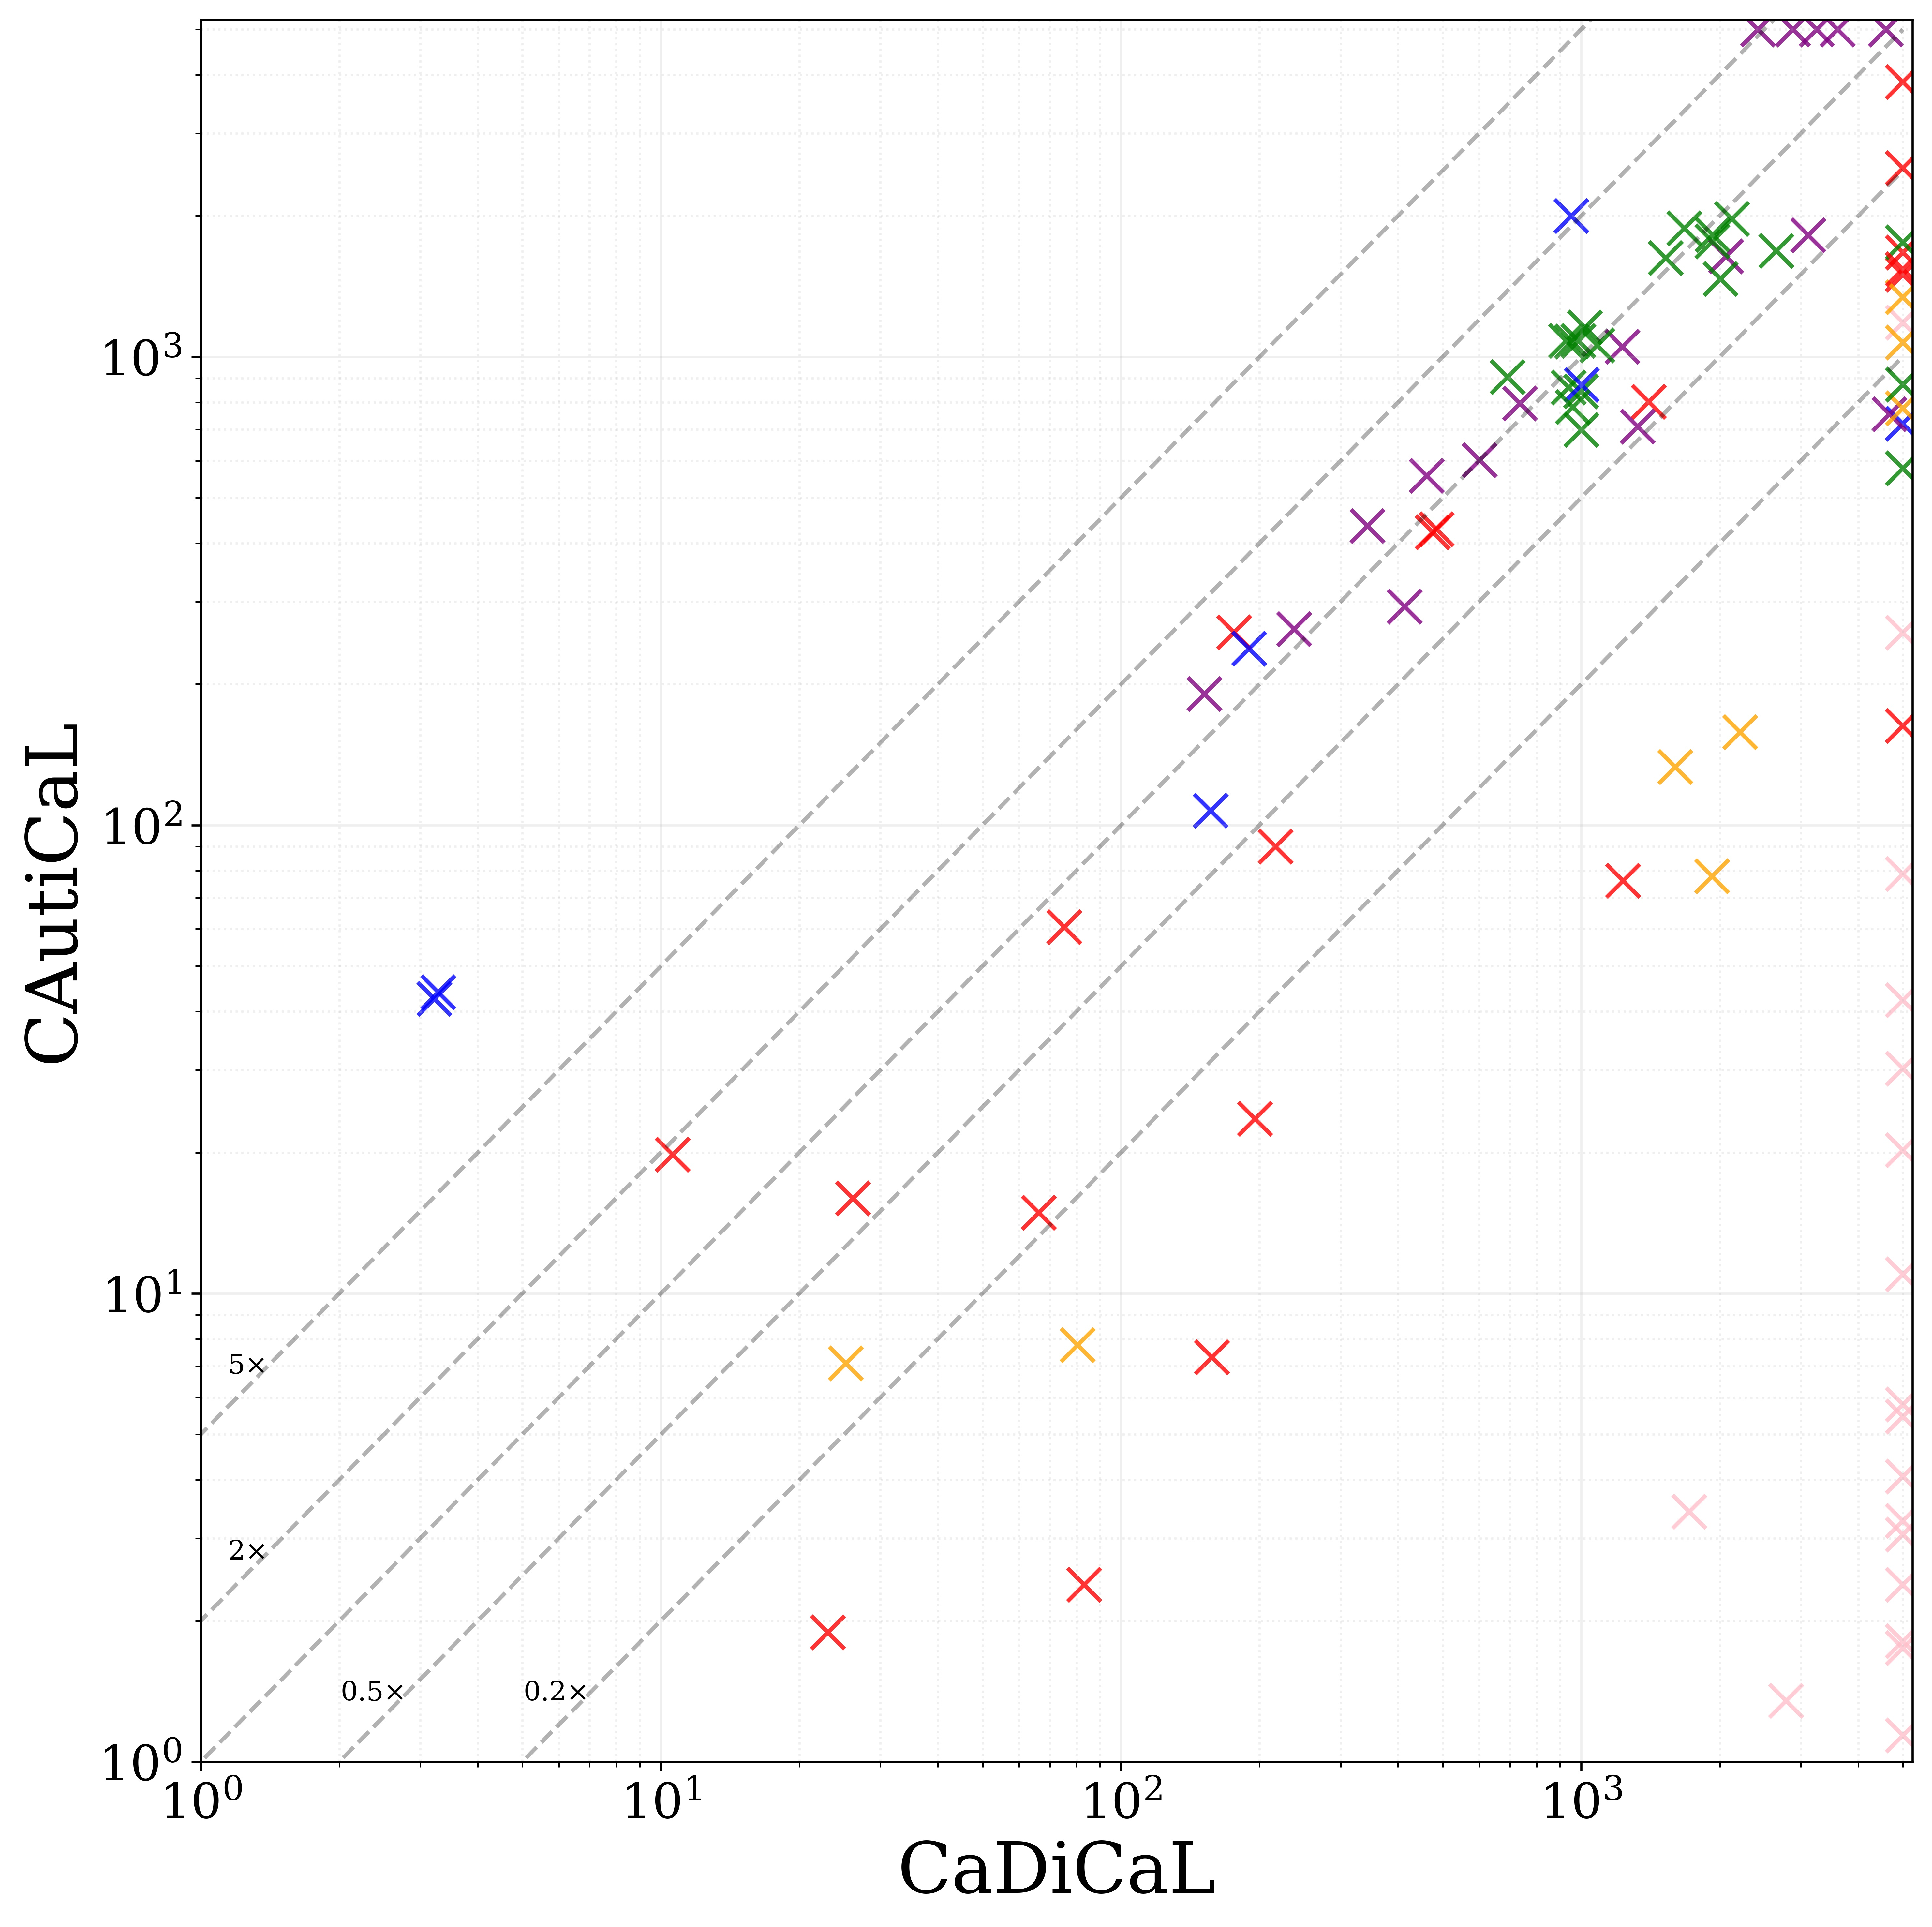
\includegraphics[width=\textwidth]{figs/cadical_vs_cautical_interesting.jpg}
            \caption{Comparison with \cadical}
            \label{fig:cautical-vs-cadical}
    \end{subfigure}
        % \hspace{0.06\textwidth}
    % \hspace{0.06\textwidth}
    % \begin{subfigure}[t]{0.3\textwidth}
    %     \centering
    %     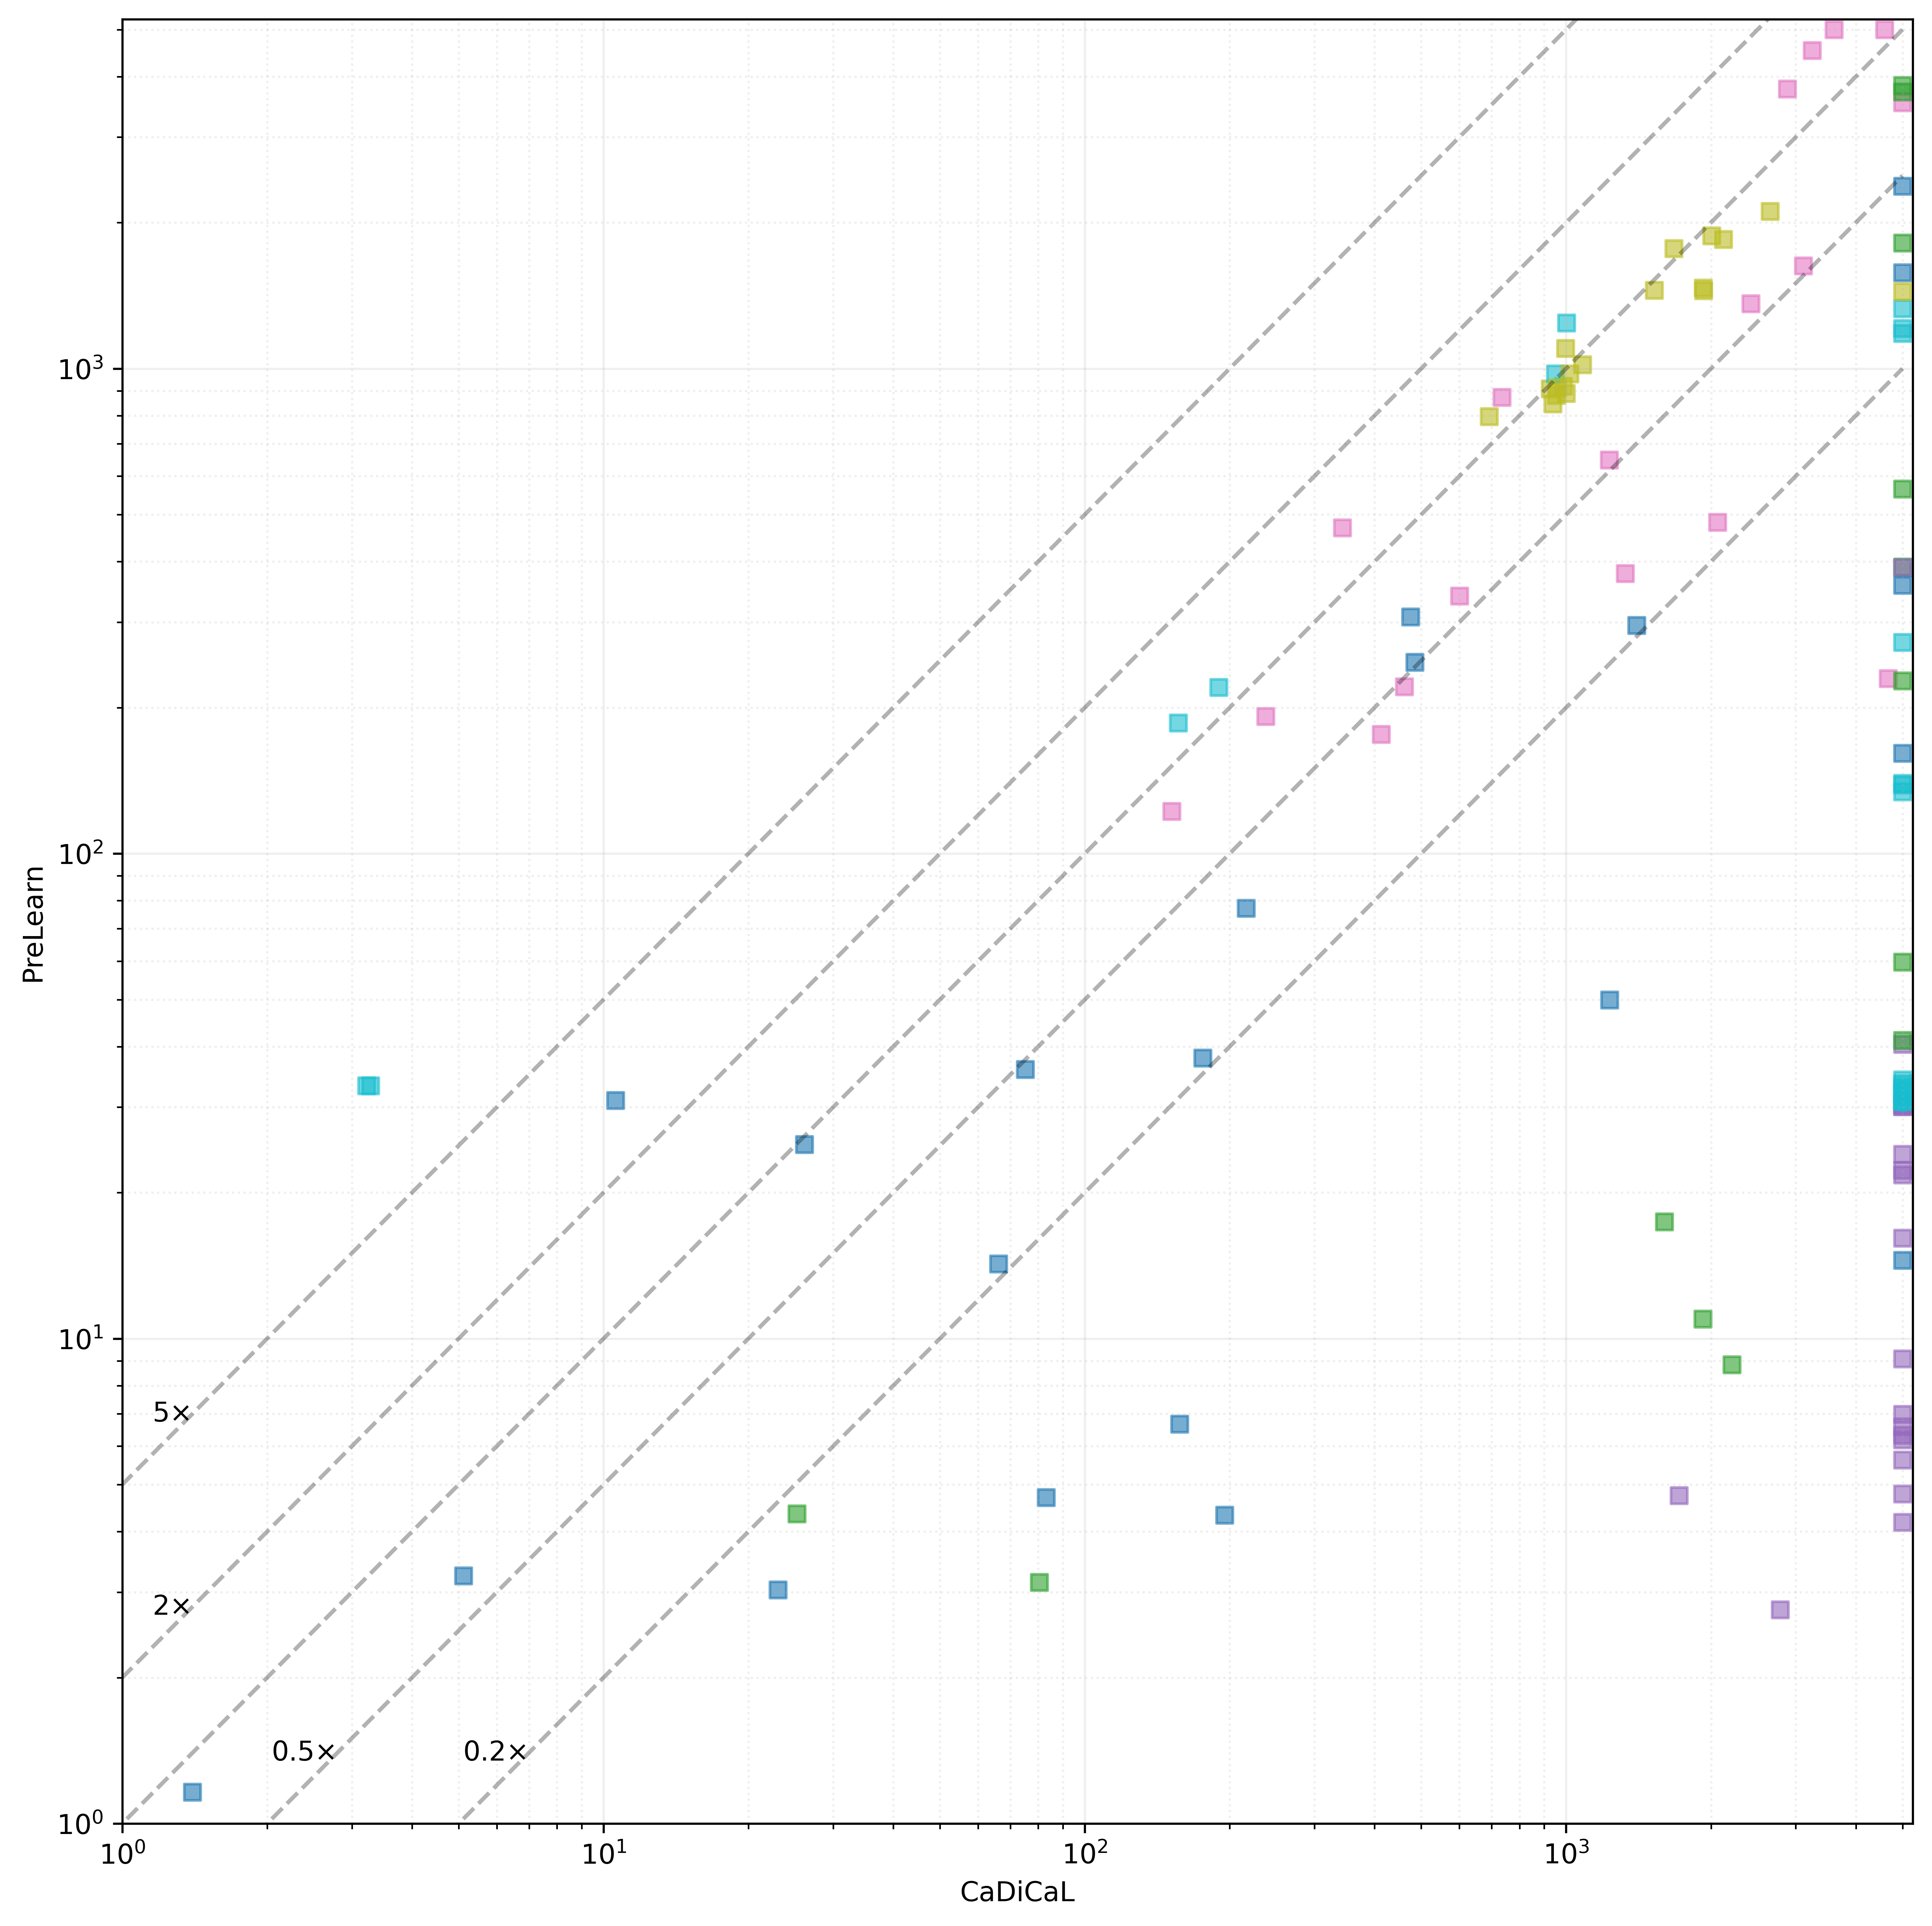
\includegraphics[width=\textwidth]{figs/prelearn_vs_cadical_interesting.jpg}
    %     \caption{Comparison with \prelearn}
    %     \label{fig:cautical-vs-prelearn}
    % \end{subfigure}
    \begin{subfigure}[t]{0.45\textwidth}
        \centering
        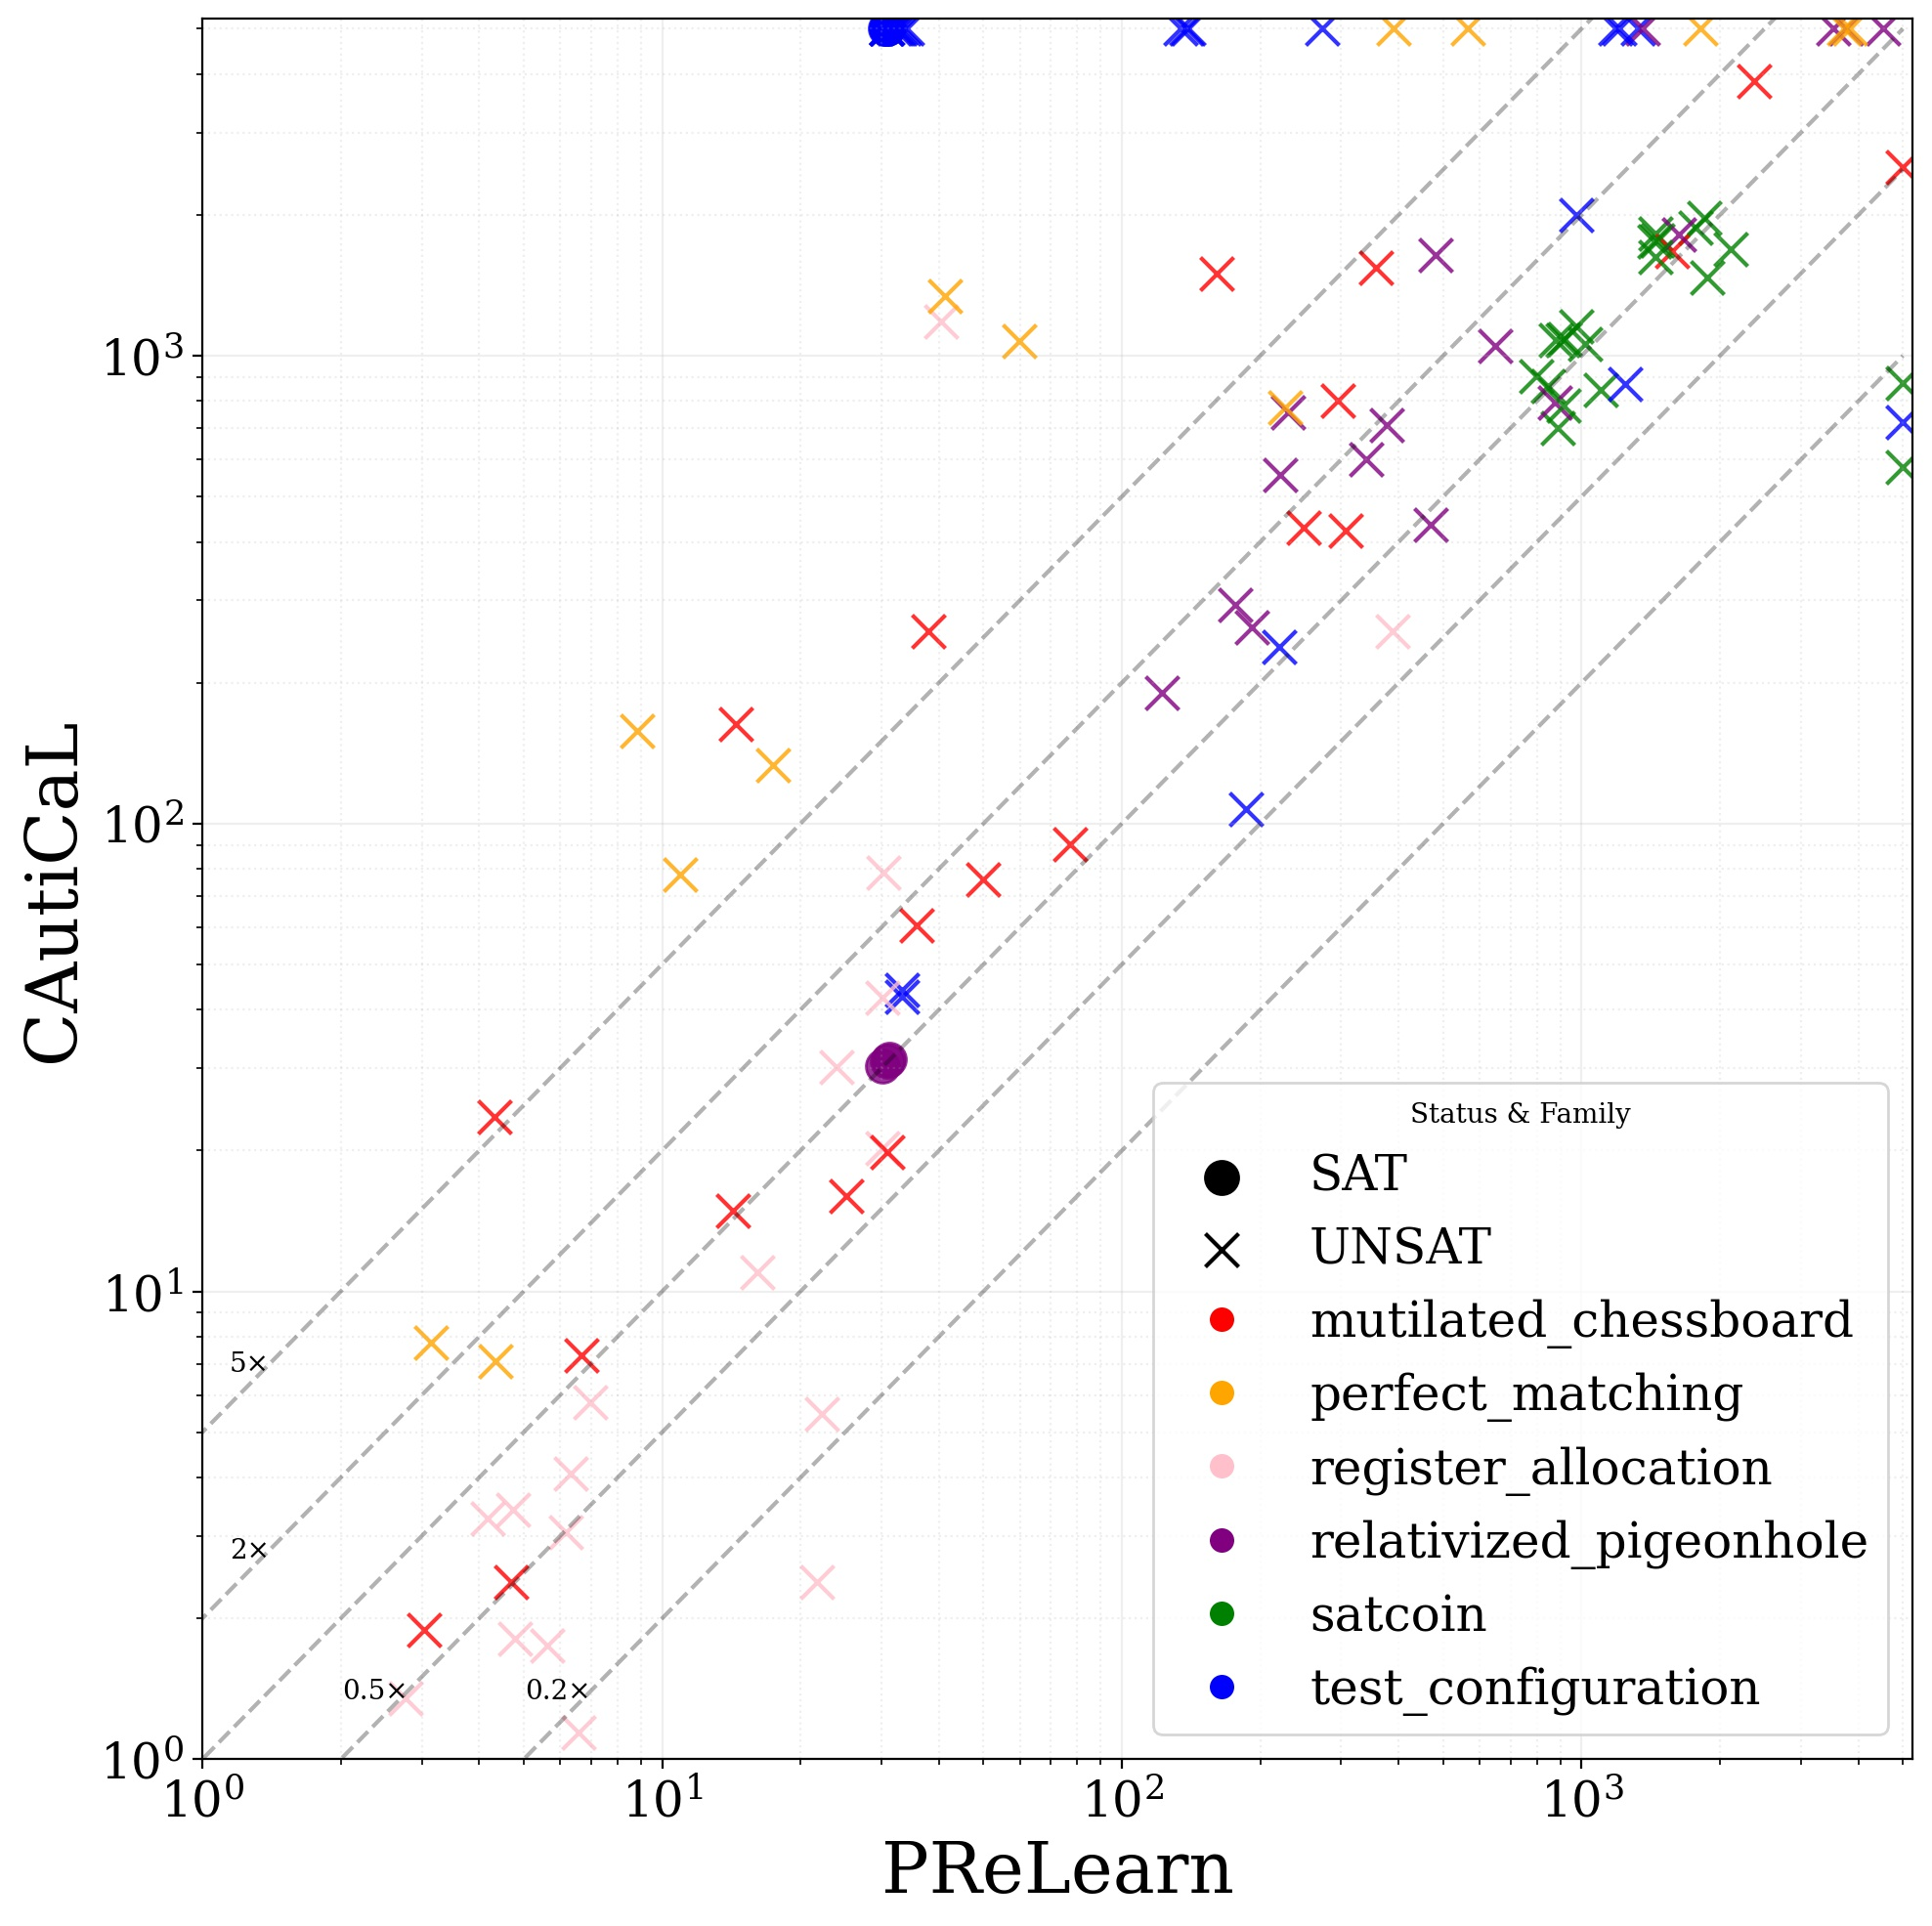
\includegraphics[width=\textwidth]{figs/prelearn_vs_cautical_interesting_legend.jpg}
        \caption{Comparison with \prelearn}
        \label{fig:cautical-vs-prelearn}
    \end{subfigure}

    \caption{Performance comparison of \tool with other solvers on benchmark families.}
    \label{fig:solver-comparison-familis}
\end{figure*}


\subsection{Analysis of heuristics}~\label{subsec:eval-heuristics}

\autoref{fig:global-heuristics} shows the performance of \tool with different heuristics turned on and off. First we consider turning three optimizations off. \autoref{fig:globaldontfilter} compares against when we turn off filtering short and non-trivial \pr clauses. \autoref{fig:global-max-length} compares against when we filter only clauses of length $10$ or greater. \autoref{fig:global-no-shrink} compares to when we decide not to shrink clauses. When we disable all three optimizations, the performance is significantly, especially on \texttt{perfect-matching}, \texttt{mutilated-chessboard}, and \texttt{register-allocation} benchmarks.

Additionally, we consider potential improvements to the heuristics used in \tool. Three possible options are to change the time limit of preprocessing, try to efficiently sort the first propagated variable $i$ and try to sort the second propagated variable $j$. \autoref{fig:global-time-limit} does the first, by setting the pre-processing time limit to 100 seconds. \autoref{fig:global-time-limit}. \autoref{fig:global-sort-i} does the second by propagating $i$ in order of which literals occurs most frequently in the original formula. Finally, \autoref{sub@fig:global-touched} does the the third, for each $i$ propagated, for each other $j$, it counts the number of clauses that contain $j$ and $i$ (or a literal propagate by $i$). It then picks $j$ based on which has the highest of this score.


%  shows that the time limit heuristic is not useful for \tool. \autoref{fig:global-sort-i} shows that sorting $i$ beforehand by frequency used is not useful. \autoref{fig:global-touched} shows that the touched heuristic is not useful.



\begin{figure*}[!t]
    \centering
    \begin{subfigure}[t]{0.3\textwidth}
        \centering
        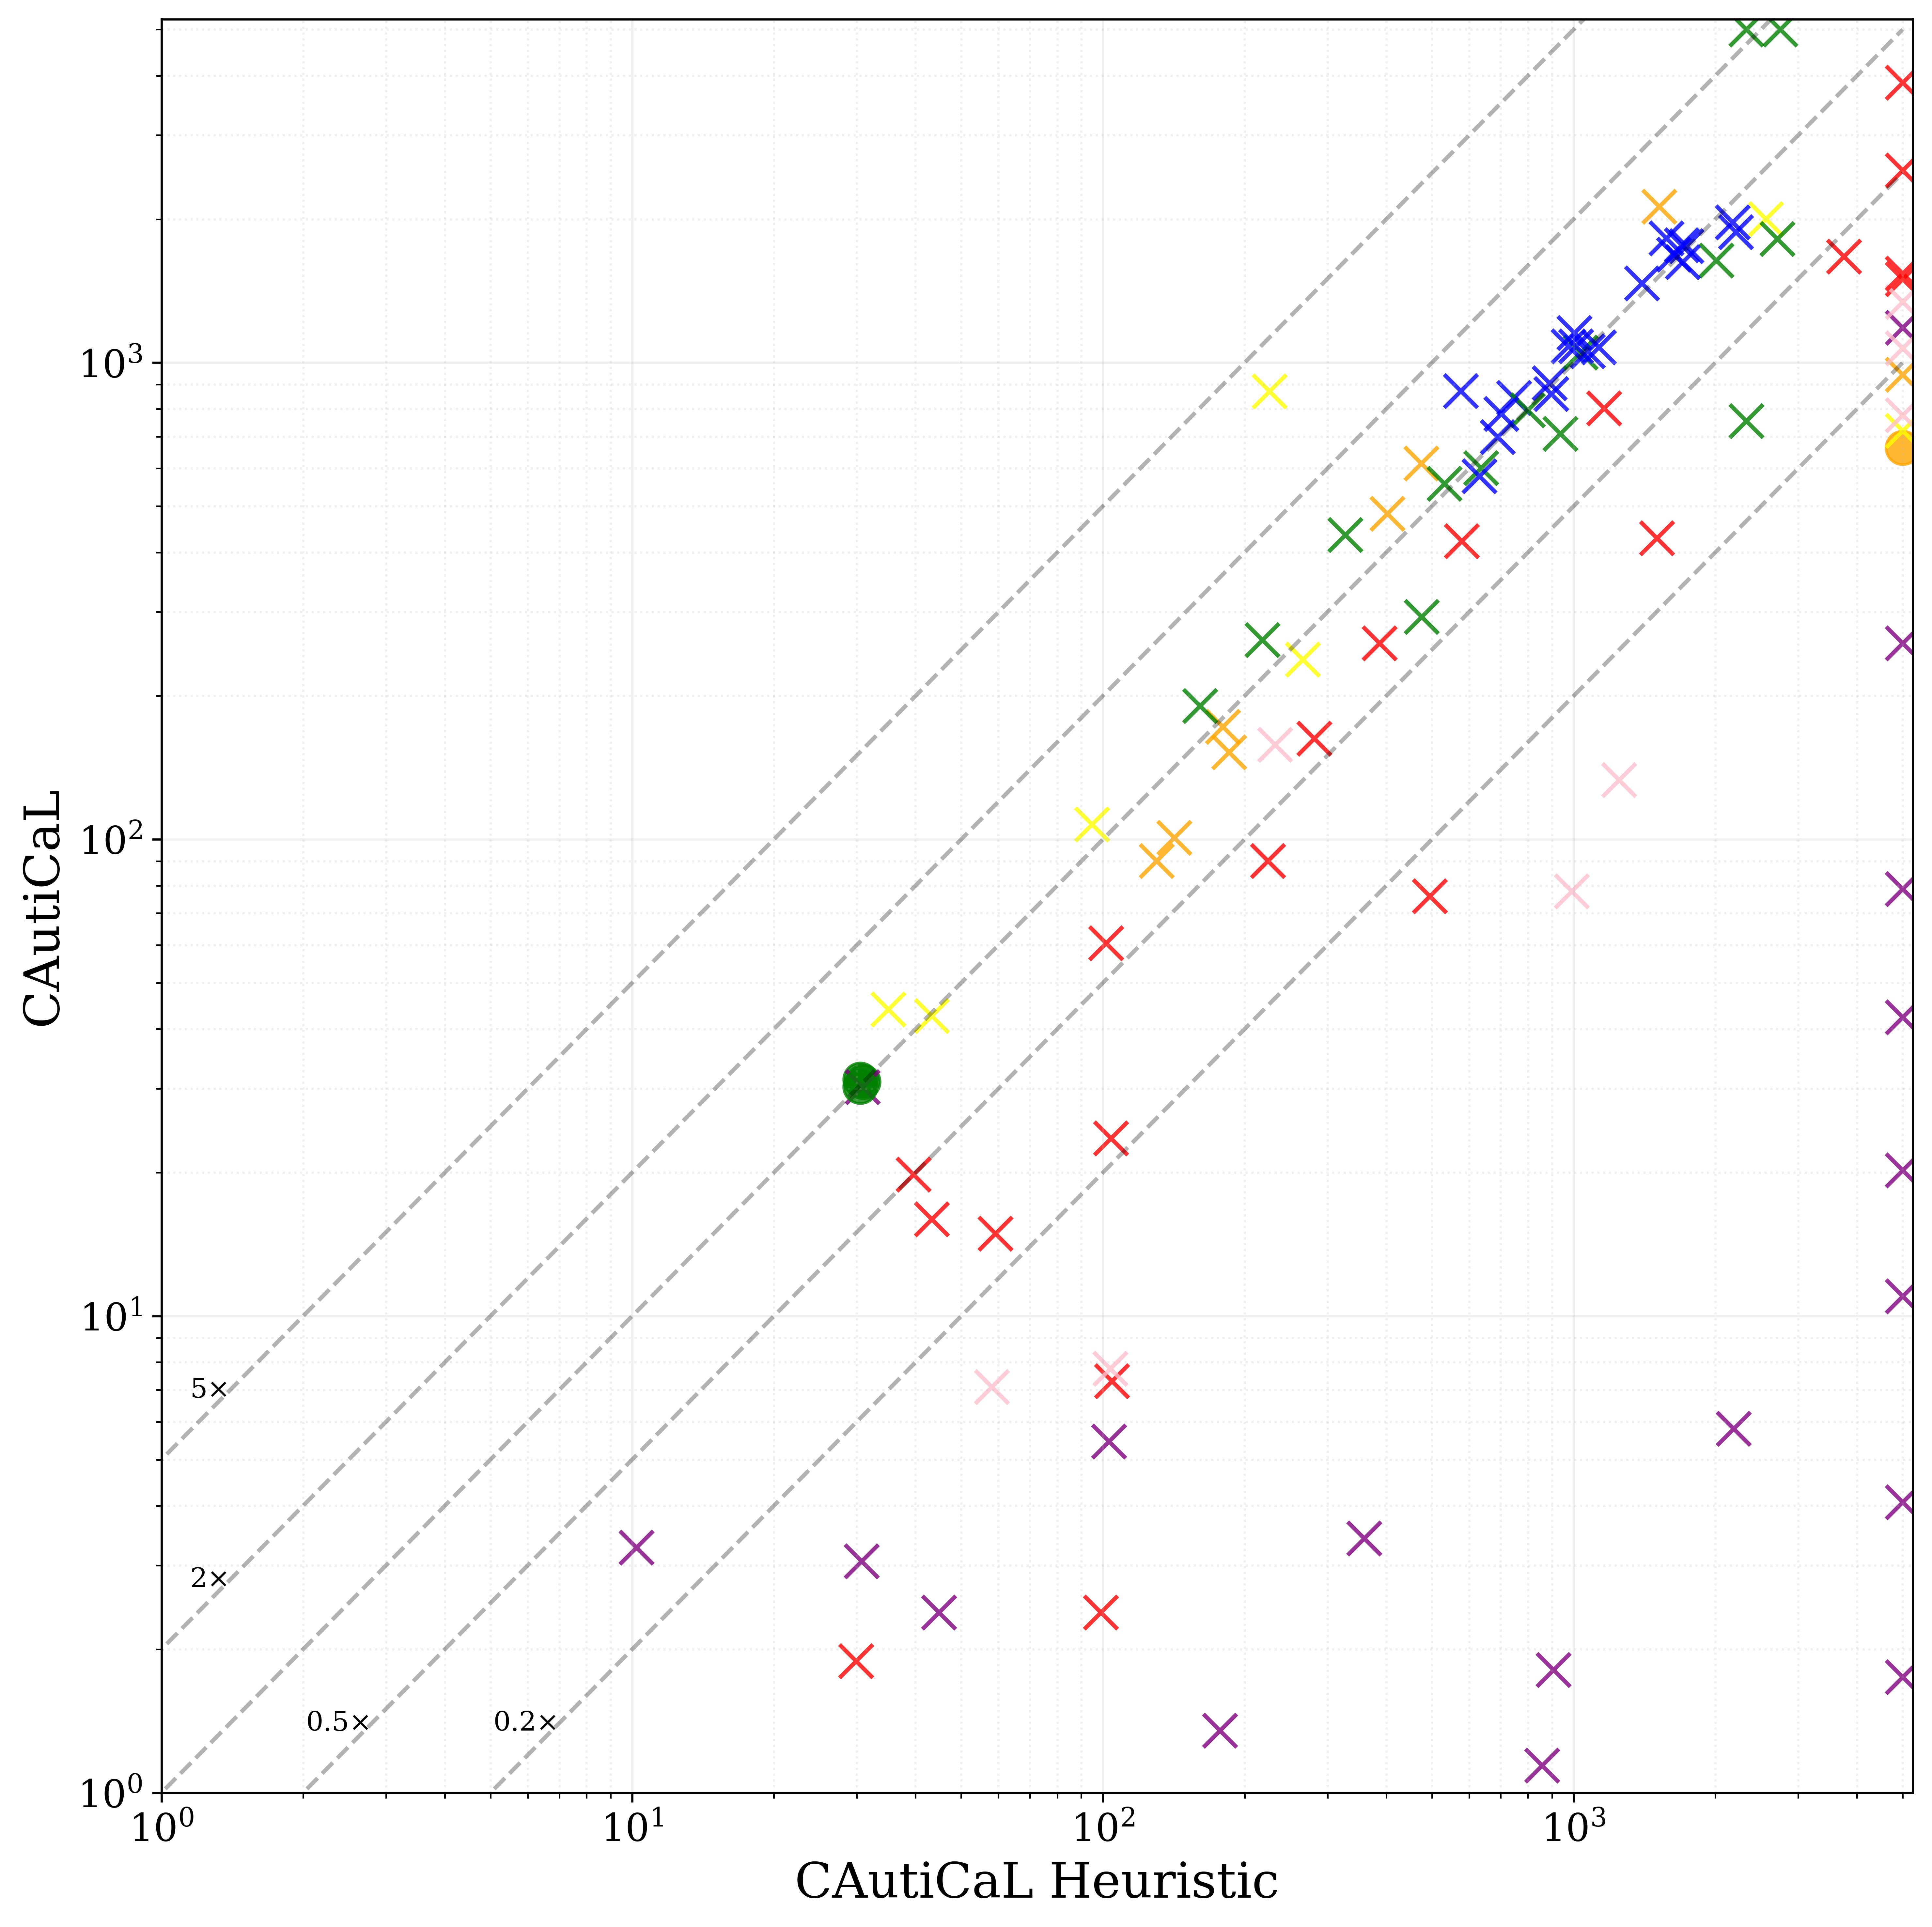
\includegraphics[width=\textwidth]{figs/globaldontfilter_heuristic_comparison.jpg}
        \caption{No filter}
        \label{fig:globaldontfilter}
    \end{subfigure}
    \begin{subfigure}[t]{0.3\textwidth}
        \centering
        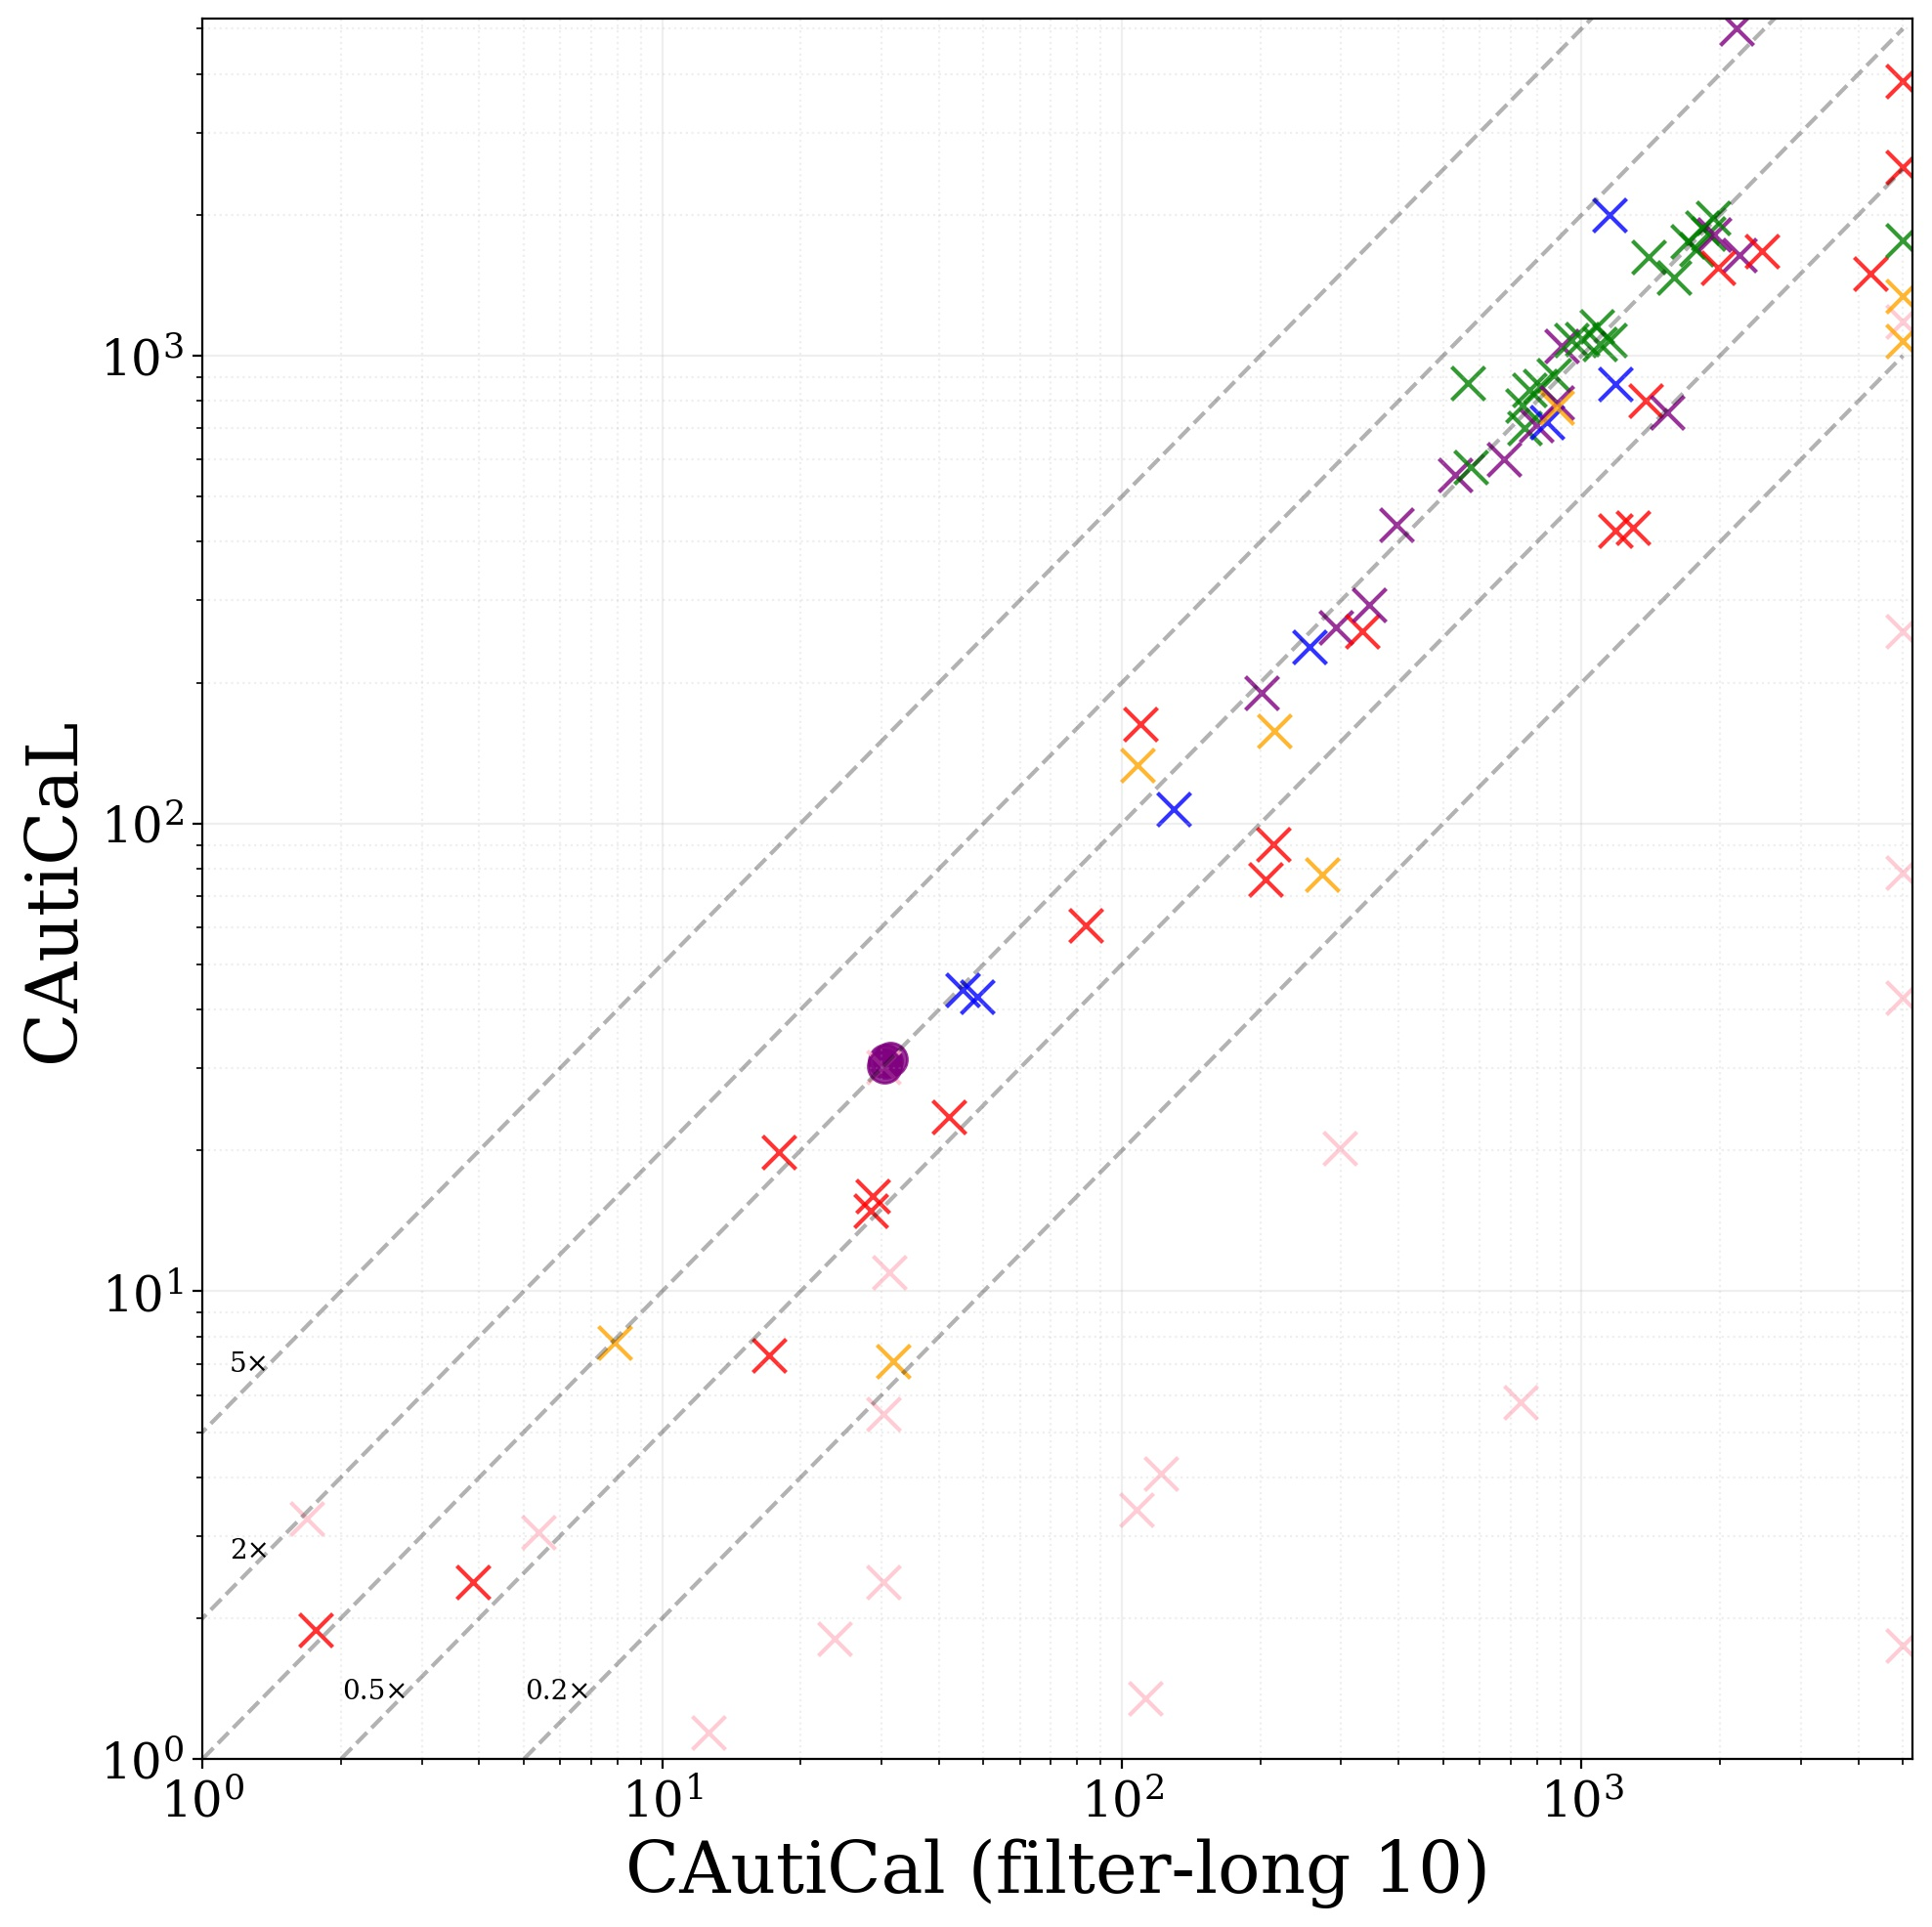
\includegraphics[width=\textwidth]{figs/globalmaxlen_heuristic_comparison.jpg}
        \caption{Max length}
        \label{fig:global-max-length}
    \end{subfigure}
    \begin{subfigure}[t]{0.3\textwidth}
            \centering
            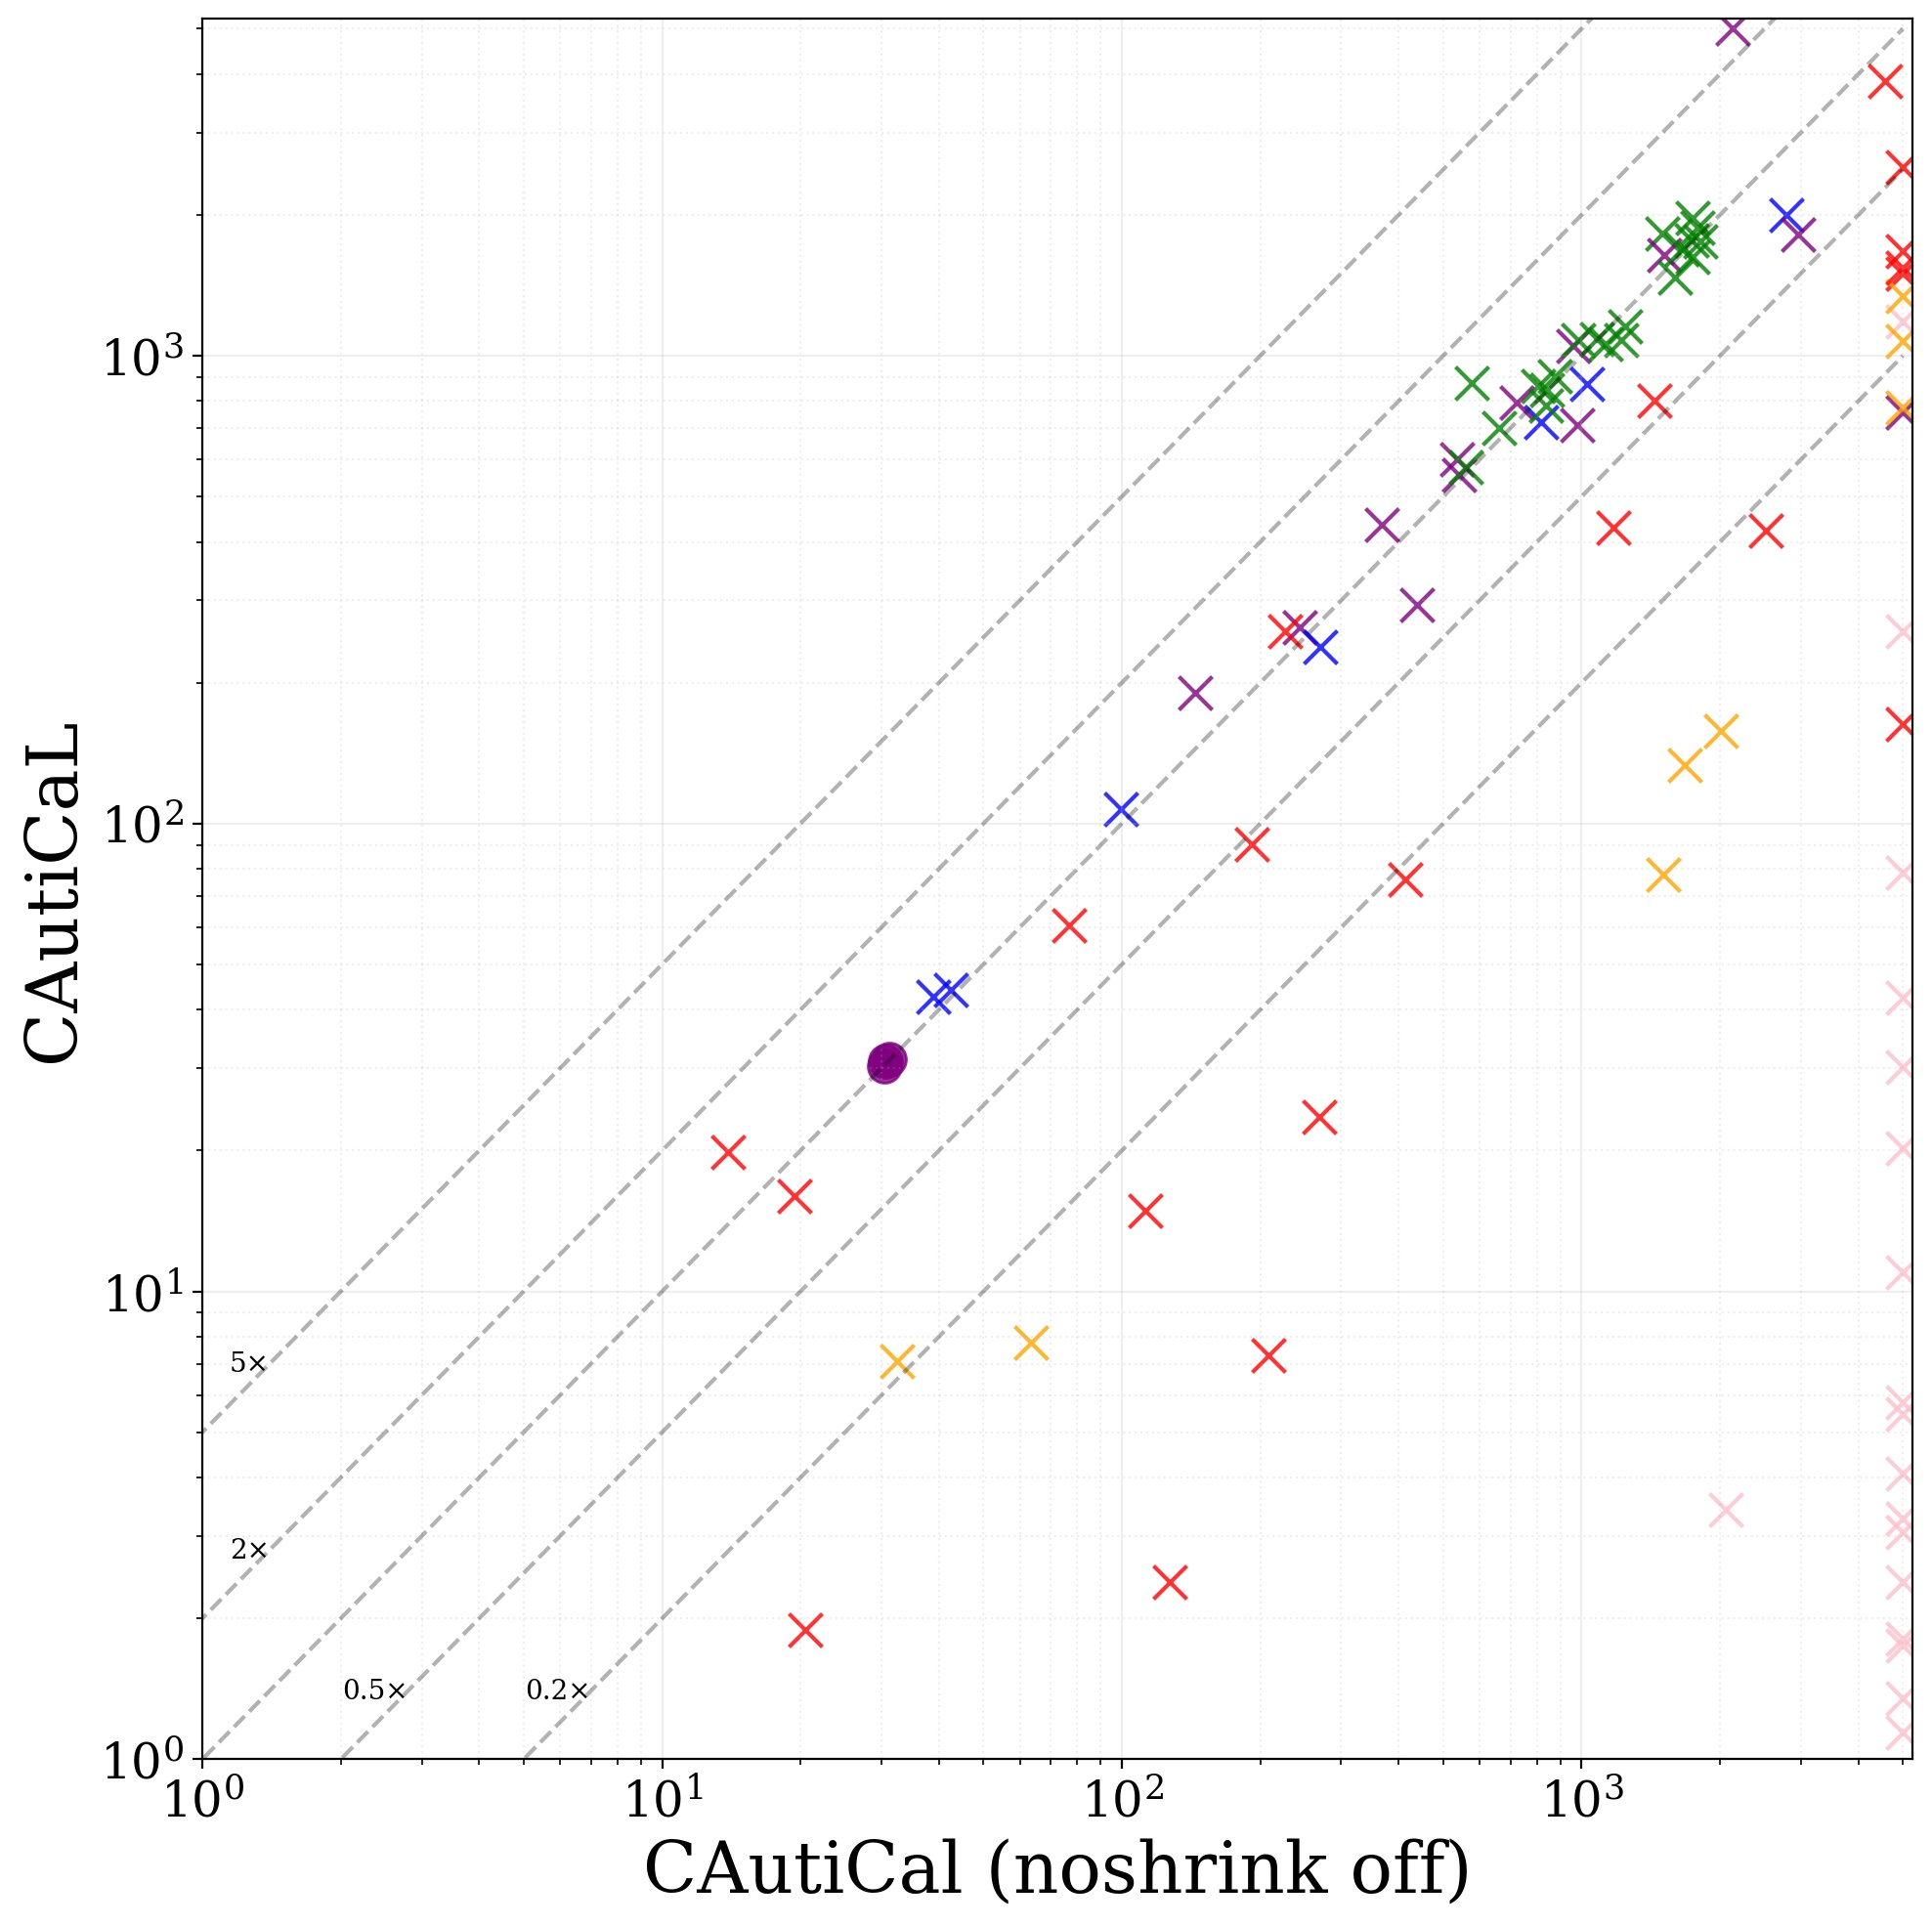
\includegraphics[width=\textwidth]{figs/globalnoshrink_heuristic_comparison.jpg}
            \caption{No shrink}
            \label{fig:global-no-shrink}
    \end{subfigure}
    \begin{subfigure}[t]{0.3\textwidth}
        \centering
        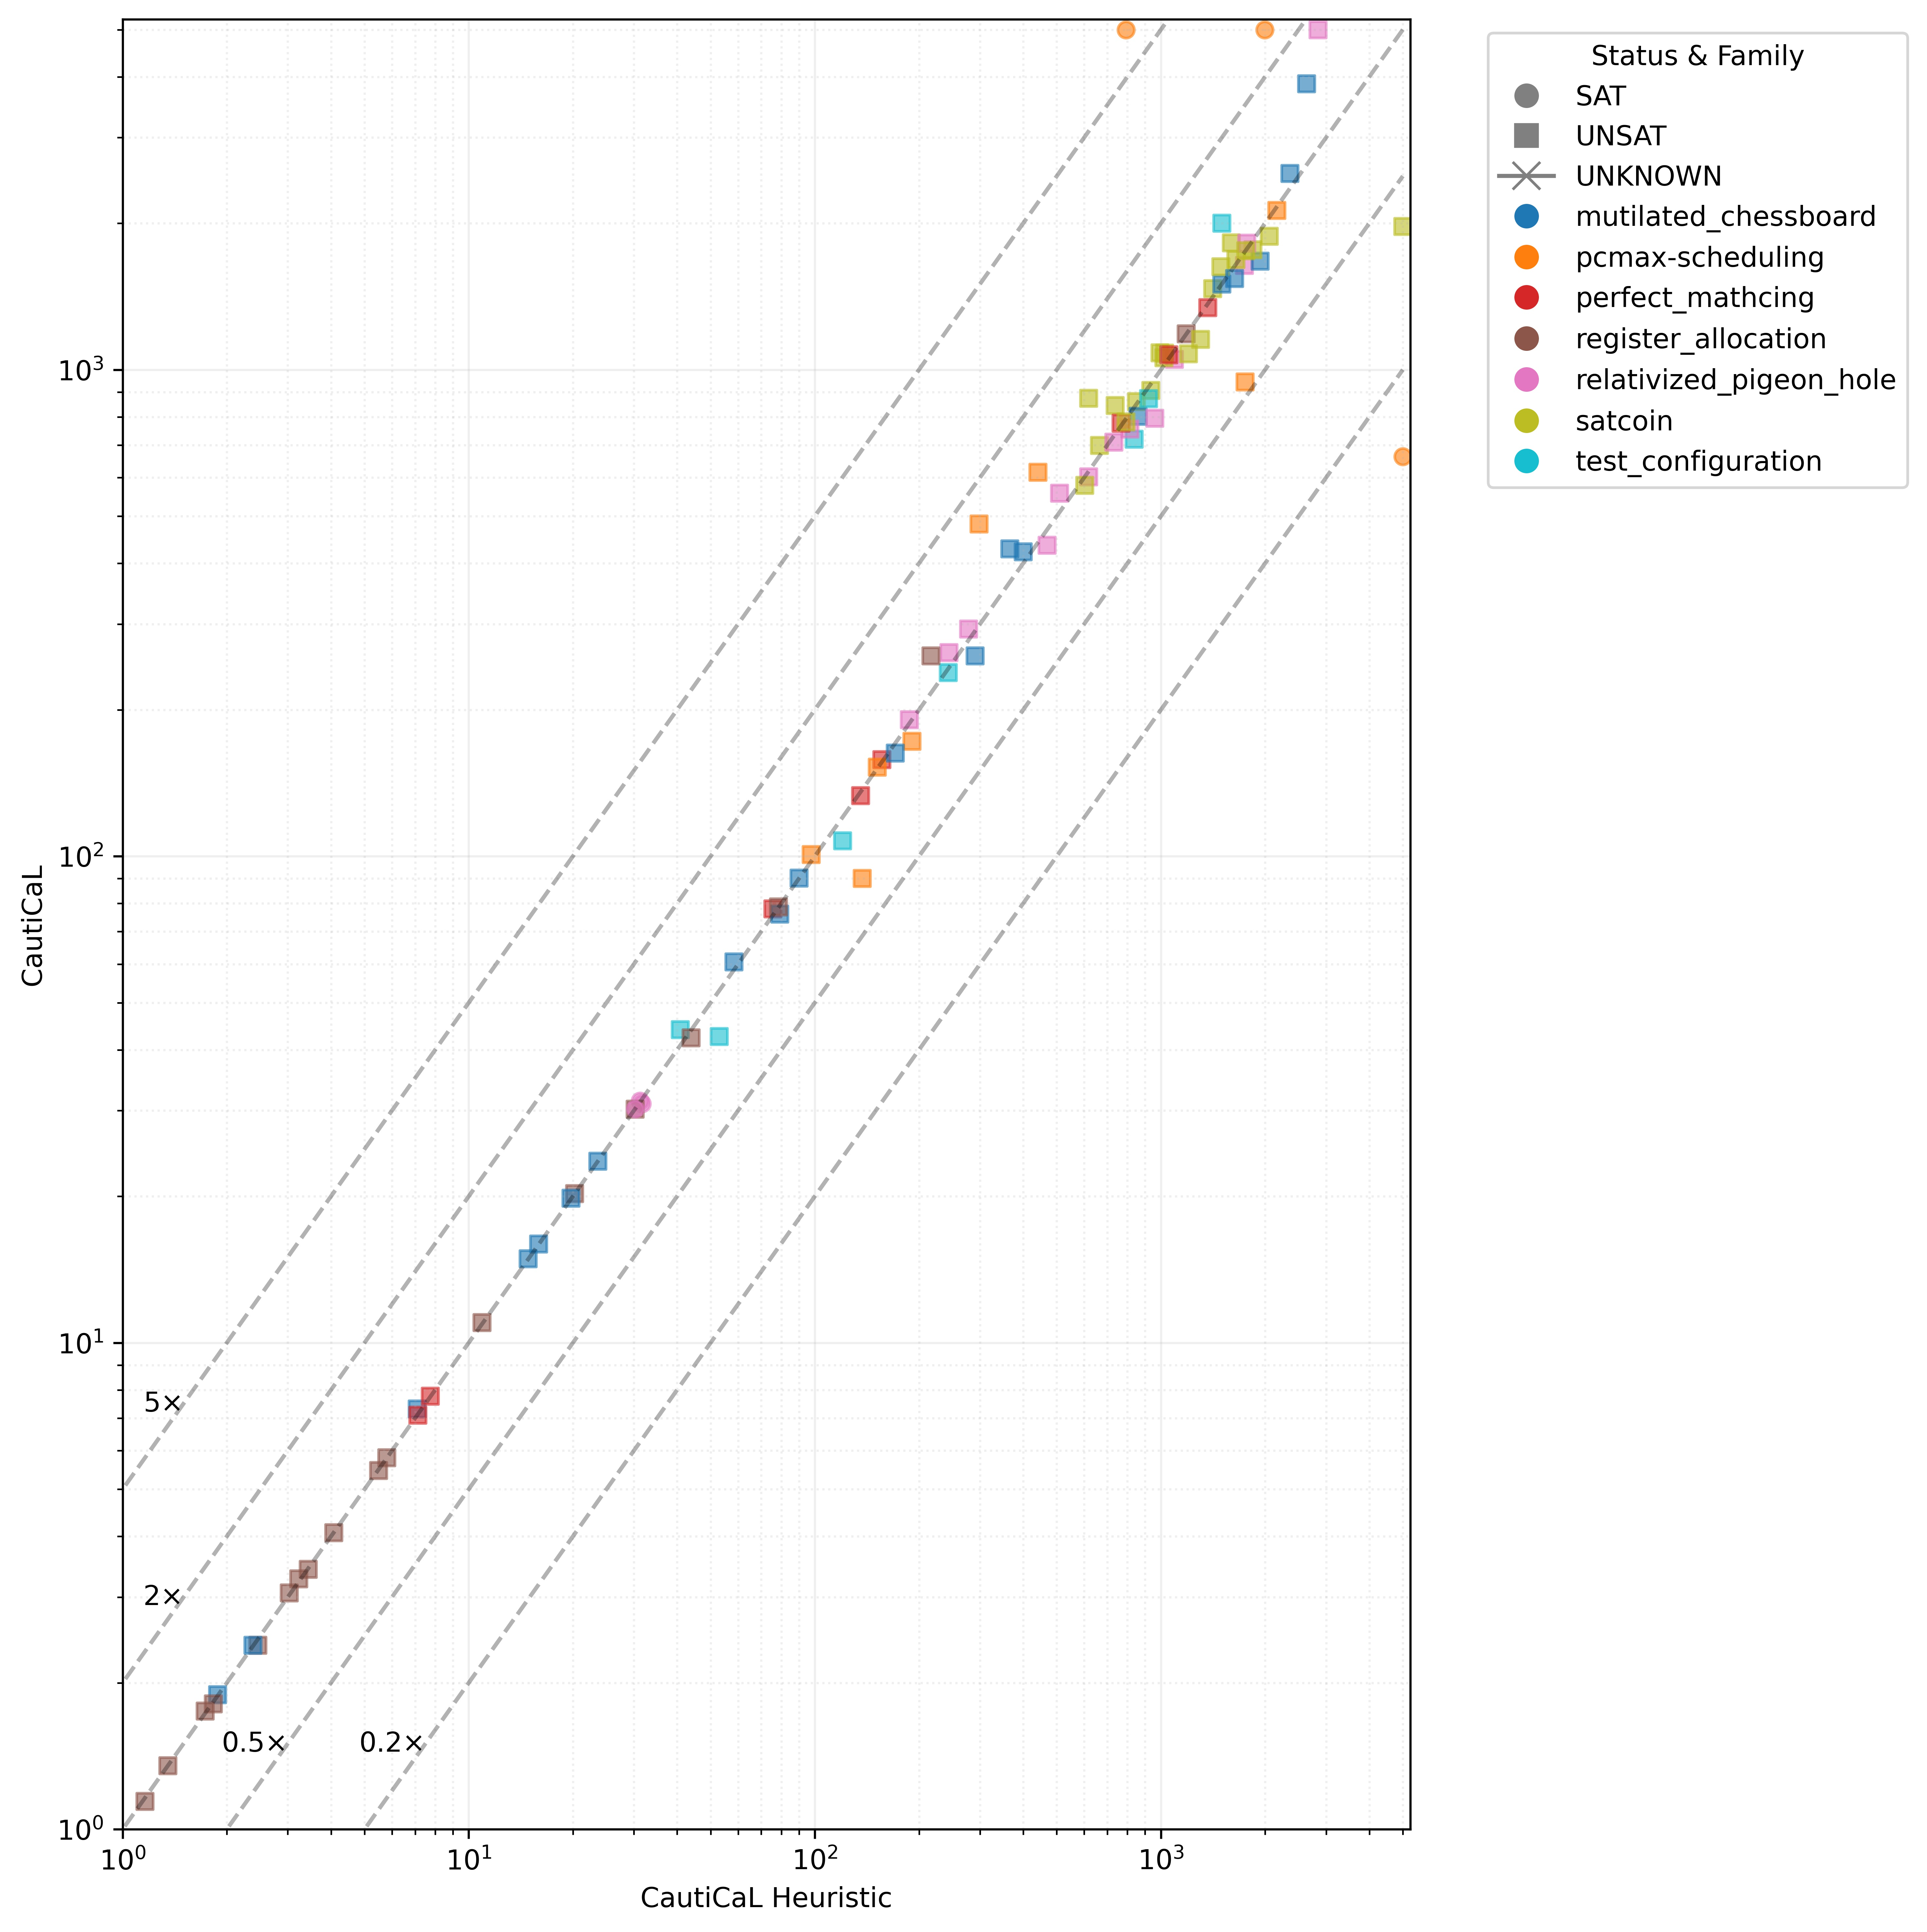
\includegraphics[width=\textwidth]{figs/global_time_lim_heuristic_comparison.jpg}
        \caption{Time limit}
        \label{fig:global-time-limit}
    \end{subfigure}
    \begin{subfigure}[t]{0.3\textwidth}
        \centering
        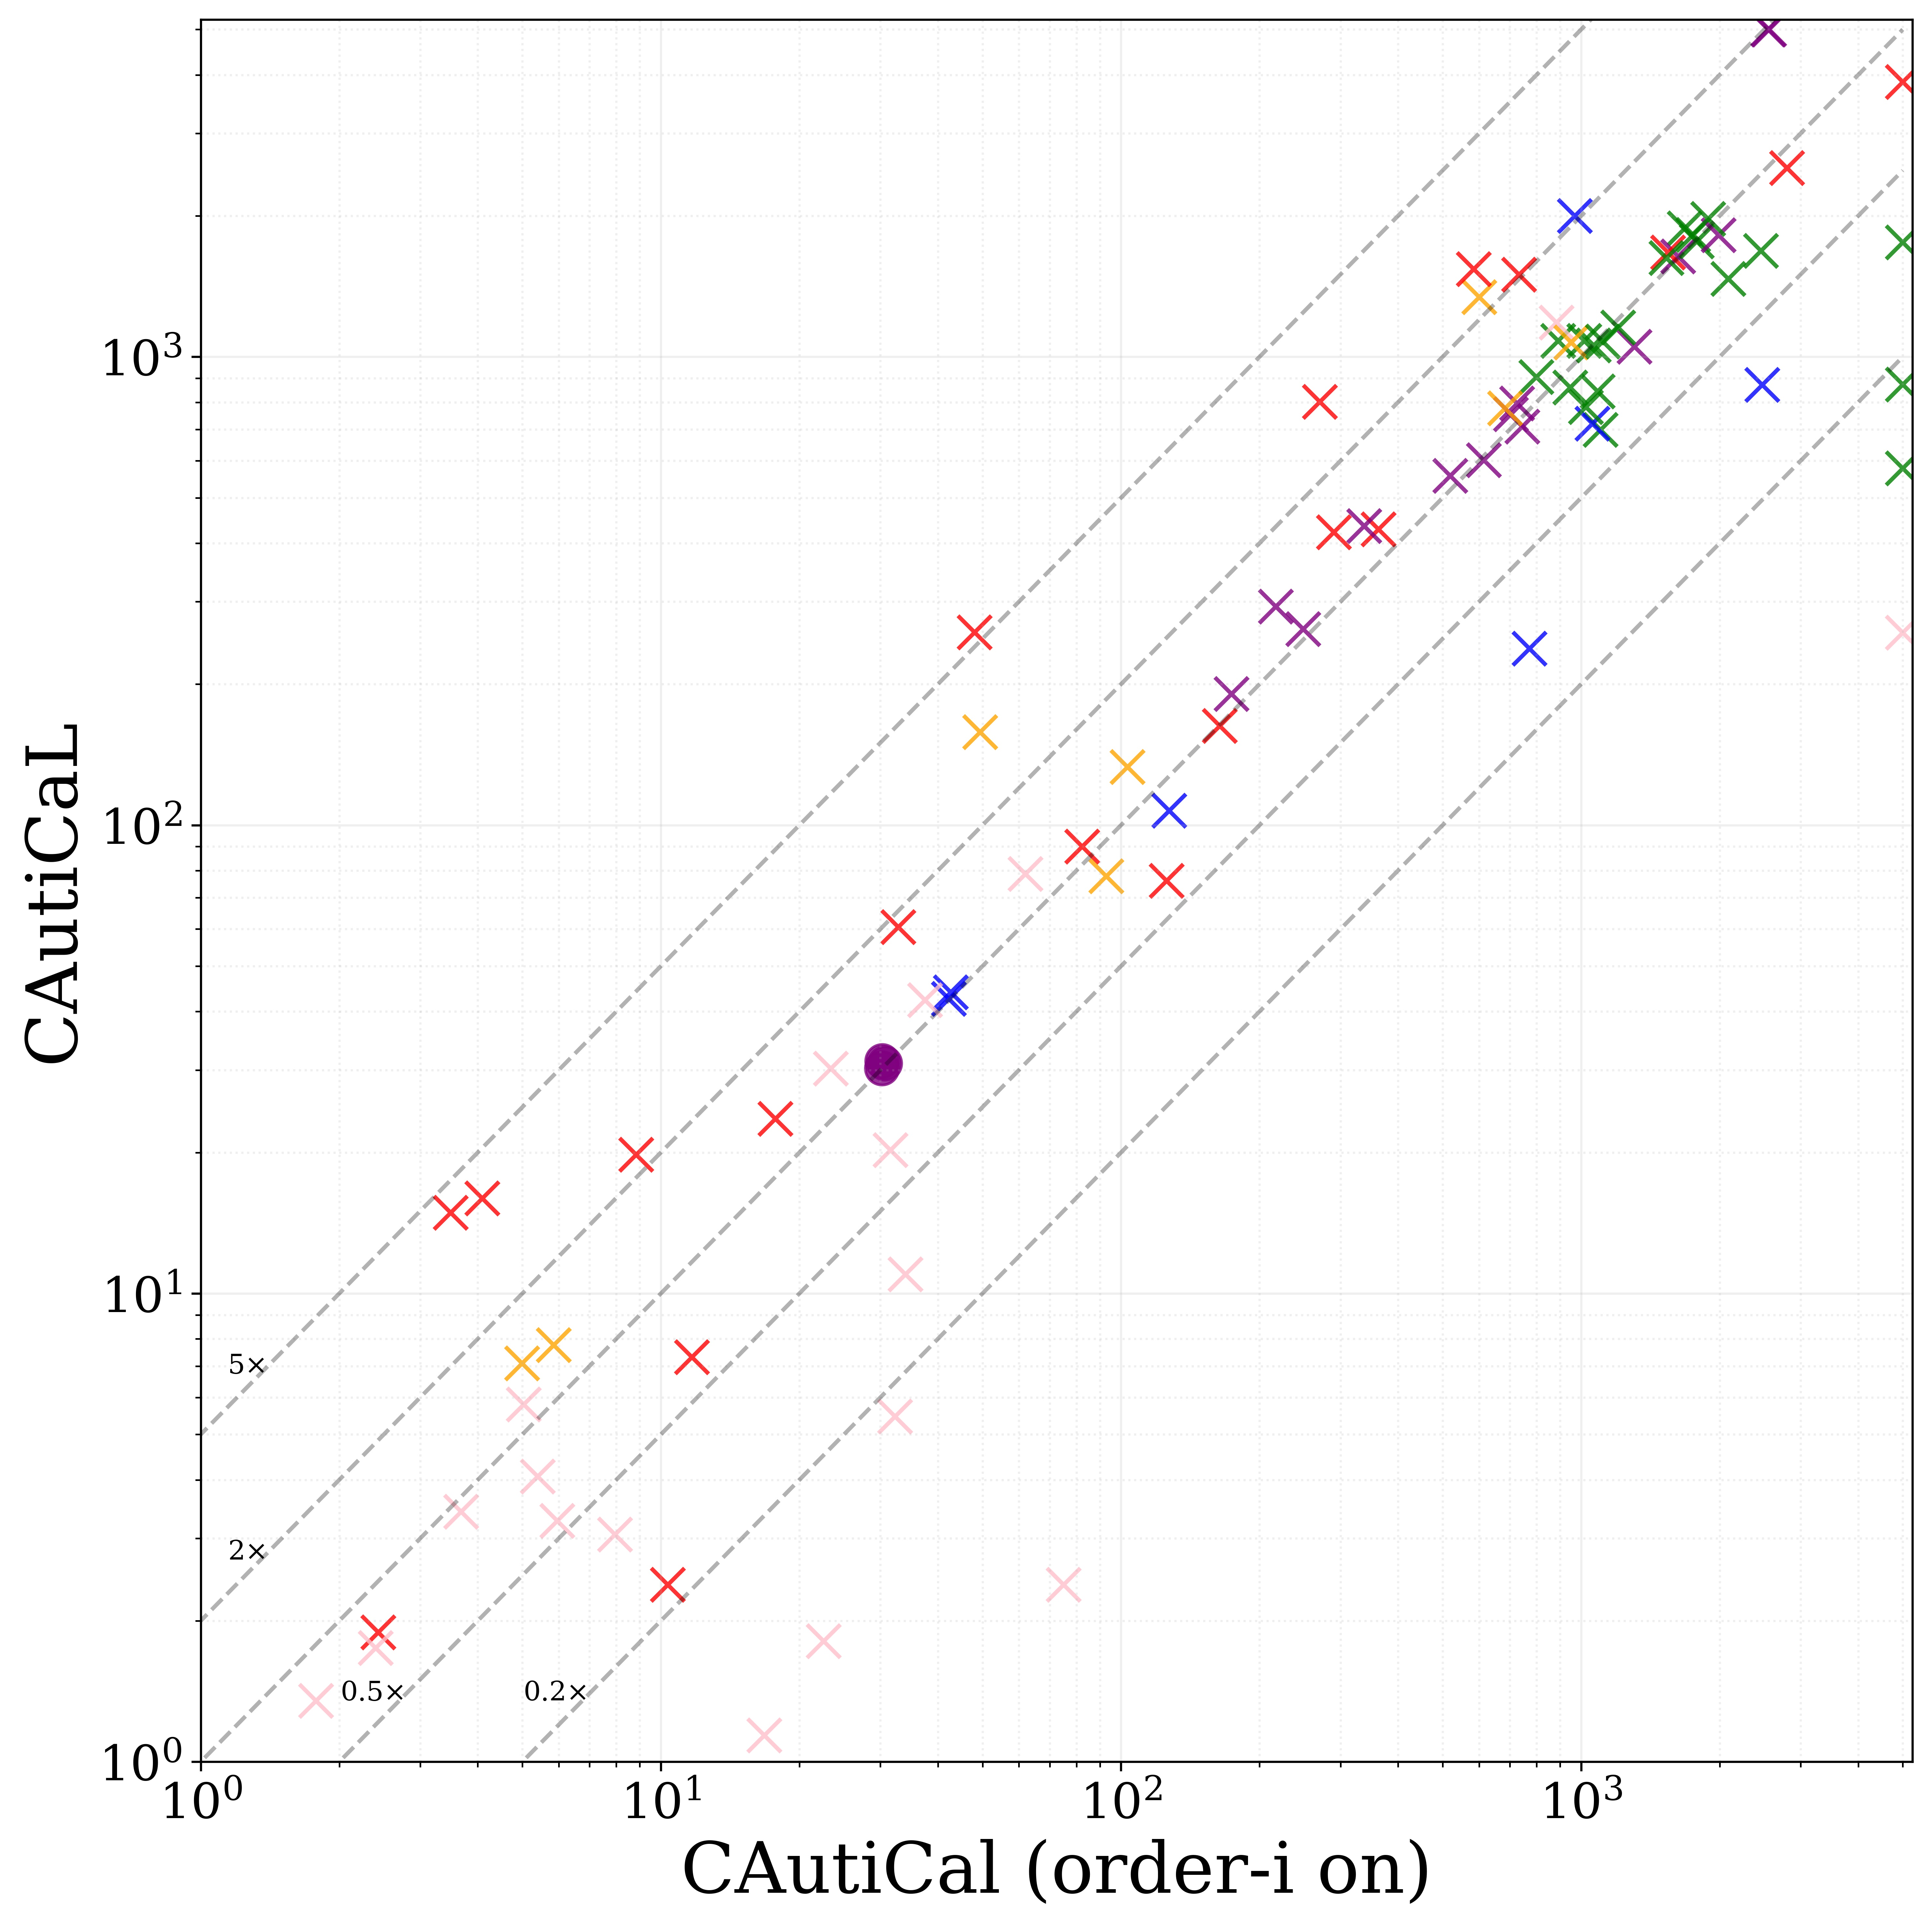
\includegraphics[width=\textwidth]{figs/globalisort_heuristic_comparison.jpg}
        \caption{Sort $i$ beforehand by frequency used}
        \label{fig:global-sort-i}
    \end{subfigure}
    \begin{subfigure}[t]{0.3\textwidth}
        \centering
        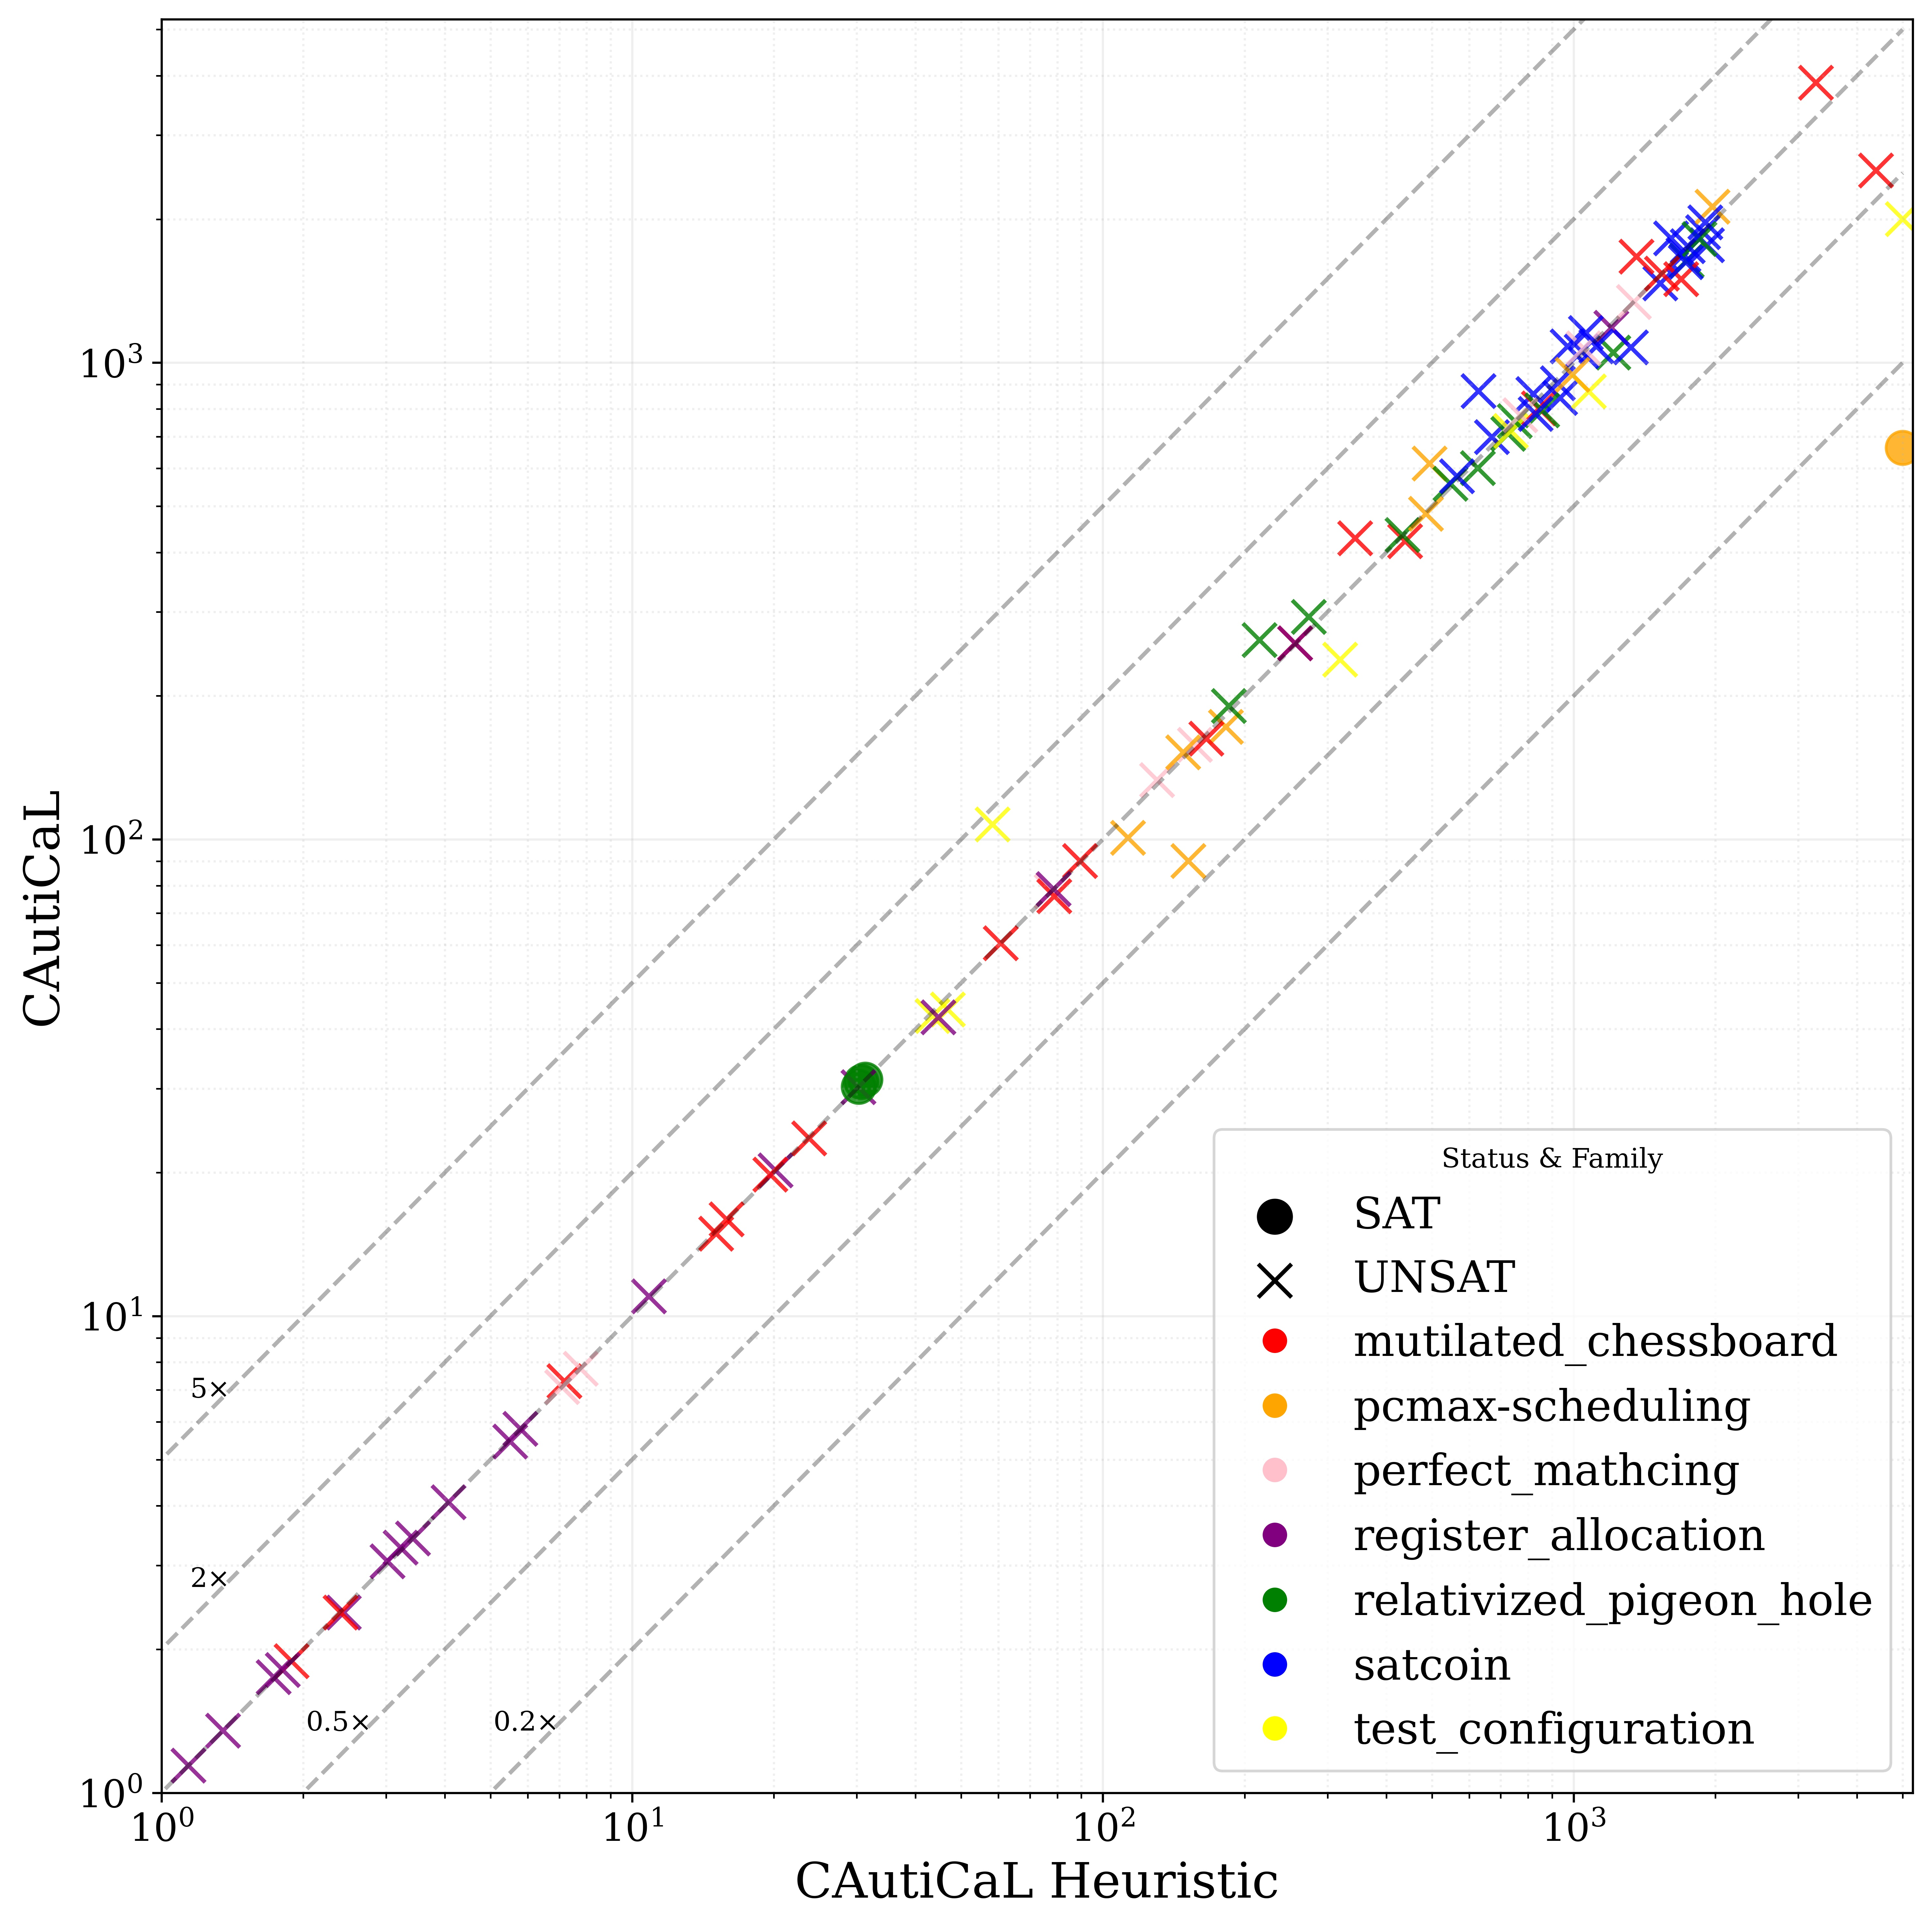
\includegraphics[width=\textwidth]{figs/globaltouch_heuristic_comparison.jpg}
        \caption{Touched heuristic}
        \label{fig:global-touched}
    \end{subfigure}
    \caption{Performance comparison of \tool with other solvers}
\end{figure*}


% \subsection{Research Questions}~\label{subsec:eval-research-questions}

